\documentclass[runningheads]{llncs}

% ---------------------------------------------------------------
% Include basic ECCV package
 
% TODO REVIEW: Insert your submission number below by replacing '*****'
% TODO FINAL: Comment out the following line for the camera-readxy version
\usepackage[review,year=2026,ID=*****]{eccv}
% TODO FINAL: Un-comment the following line for the camera-ready version
%\usepackage{eccv}

% OPTIONAL: Un-comment the following line for a version which is easier to read
% on small portrait-orientation screens (e.g., mobile phones, or beside other windows)
%\usepackage[mobile]{eccv}

\usepackage{eccvabbrv}

% Include other packages here, before hyperref.
\usepackage{graphicx}
\usepackage{todonotes}
\usepackage{booktabs}
\usepackage{multirow}
\usepackage{ulem}

% The "axessiblity" package can be found at: https://ctan.org/pkg/axessibility?lang=en
\usepackage[accsupp]{axessibility}  % Improves PDF readability for those with disabilities.


% ---------------------------------------------------------------
% Hyperref package

% It is strongly recommended to use hyperref, especially for the review version.
% Please disable hyperref *only* if you encounter grave issues.
% hyperref with option pagebackref eases the reviewers' job, but should be disabled for the final version.
%
% If you comment hyperref and then uncomment it, you should delete
% main.aux before re-running LaTeX.
% (Or just hit 'q' on the first LaTeX run, let it finish, and you
%  should be clear).

% TODO FINAL: Comment out the following line for the camera-ready version
%\usepackage[pagebackref,breaklinks,colorlinks,citecolor=eccvblue]{hyperref}
% TODO FINAL: Un-comment the following line for the camera-ready version
\usepackage{hyperref}

% Support for ORCID icon
\usepackage{orcidlink}



\begin{document}

% ---------------------------------------------------------------
% TODO REVIEW: Replace with your title
\title{SteerViT: Steering Visual Representations with Text} 

% TODO REVIEW: If the paper title is too long for the running head, you can set
% an abbreviated paper title here. If not, comment out.
\titlerunning{Abbreviated paper title}

% TODO FINAL: Replace with your author list. 
% Include the authors' OCRID for the camera-ready version, if at all possible.
\author{First Author\inst{1}\orcidlink{0000-1111-2222-3333} \and
Second Author\inst{2,3}\orcidlink{1111-2222-3333-4444} \and
Third Author\inst{3}\orcidlink{2222--3333-4444-5555}}

% TODO FINAL: Replace with an abbreviated list of authors.
\authorrunning{F.~Author et al.}
% First names are abbreviated in the running head.
% If there are more than two authors, 'et al.' is used.

% TODO FINAL: Replace with your institution list.
\institute{Princeton University, Princeton NJ 08544, USA \and
Springer Heidelberg, Tiergartenstr.~17, 69121 Heidelberg, Germany
\email{lncs@springer.com}\\
\url{http://www.springer.com/gp/computer-science/lncs} \and
ABC Institute, Rupert-Karls-University Heidelberg, Heidelberg, Germany\\
\email{\{abc,lncs\}@uni-heidelberg.de}}

\maketitle

% intro
% related work
    % general directions for steering / influencing visual features
    % elip, personalized | vlm
    % flare (?) (late fusion)
    % some weird "swan" image -- Manu
% method text-conditioned visual
    % architecture modifications
    % datasets + training signals
    % inference-time text conditioning
% experiments (hypothesis validating) ## arxiv - before method
    % conditional retrieval kNN
        % baseline: late fusion
    % without losing classification
        % pareto explain
    % attention does steer to text descriptions (results by segmentation)
% analysis / applications
    % personalized: how to condition (PODS)
    % anomaly detection
    % where are my keys (?)
    % (???) hallucination detection, negation 
    % (???) VQA
% ablations / features of our approach -- justifying choices of method (a subset of task)
    % architecture (sigmoid gating, FFN block, CA blocks)
    % backbones (MAE, SigLIP) (?)
    % scale the model (ViT-L)
    % losses (?)
    % resolution (?)
    % token length [optional!]
% conclusion



\begin{abstract}
Pretrained Vision Transformers exhibit a \textit{saliency bias}: their features collapse toward the most prominent objects in a scene, ignoring task-relevant details.
Existing approaches either produce rich but unsteerable representations (e.g., DINOv2) or achieve text-guided attention at the cost of degraded feature quality (e.g., SAM2, GroundingDINO).
We introduce SHIFT, a method that inserts sparse, tanh-gated cross-attention layers into any frozen ViT trained on referential segmentation, steering both global and dense visual features with natural language while preserving the quality of the underlying representation.
SHIFT achieves a Pareto improvement over prior work: across three ViT families (DINOv2, SigLIP, MAE), it consistently outperforms query-agnostic baselines on conditional retrieval, dense prediction, and personalized object discrimination, and generalizes zero-shot to out-of-distribution domains, reaching 64.2 AuPRO on MVTec anomaly detection (vs.\ 34.0 for CLIPSeg and 48.2 for SAM2).
  \keywords{Visual Representation \and Semantic Steering \and Text-Conditioning}
\end{abstract}
\begin{figure}[t]
    \centering
    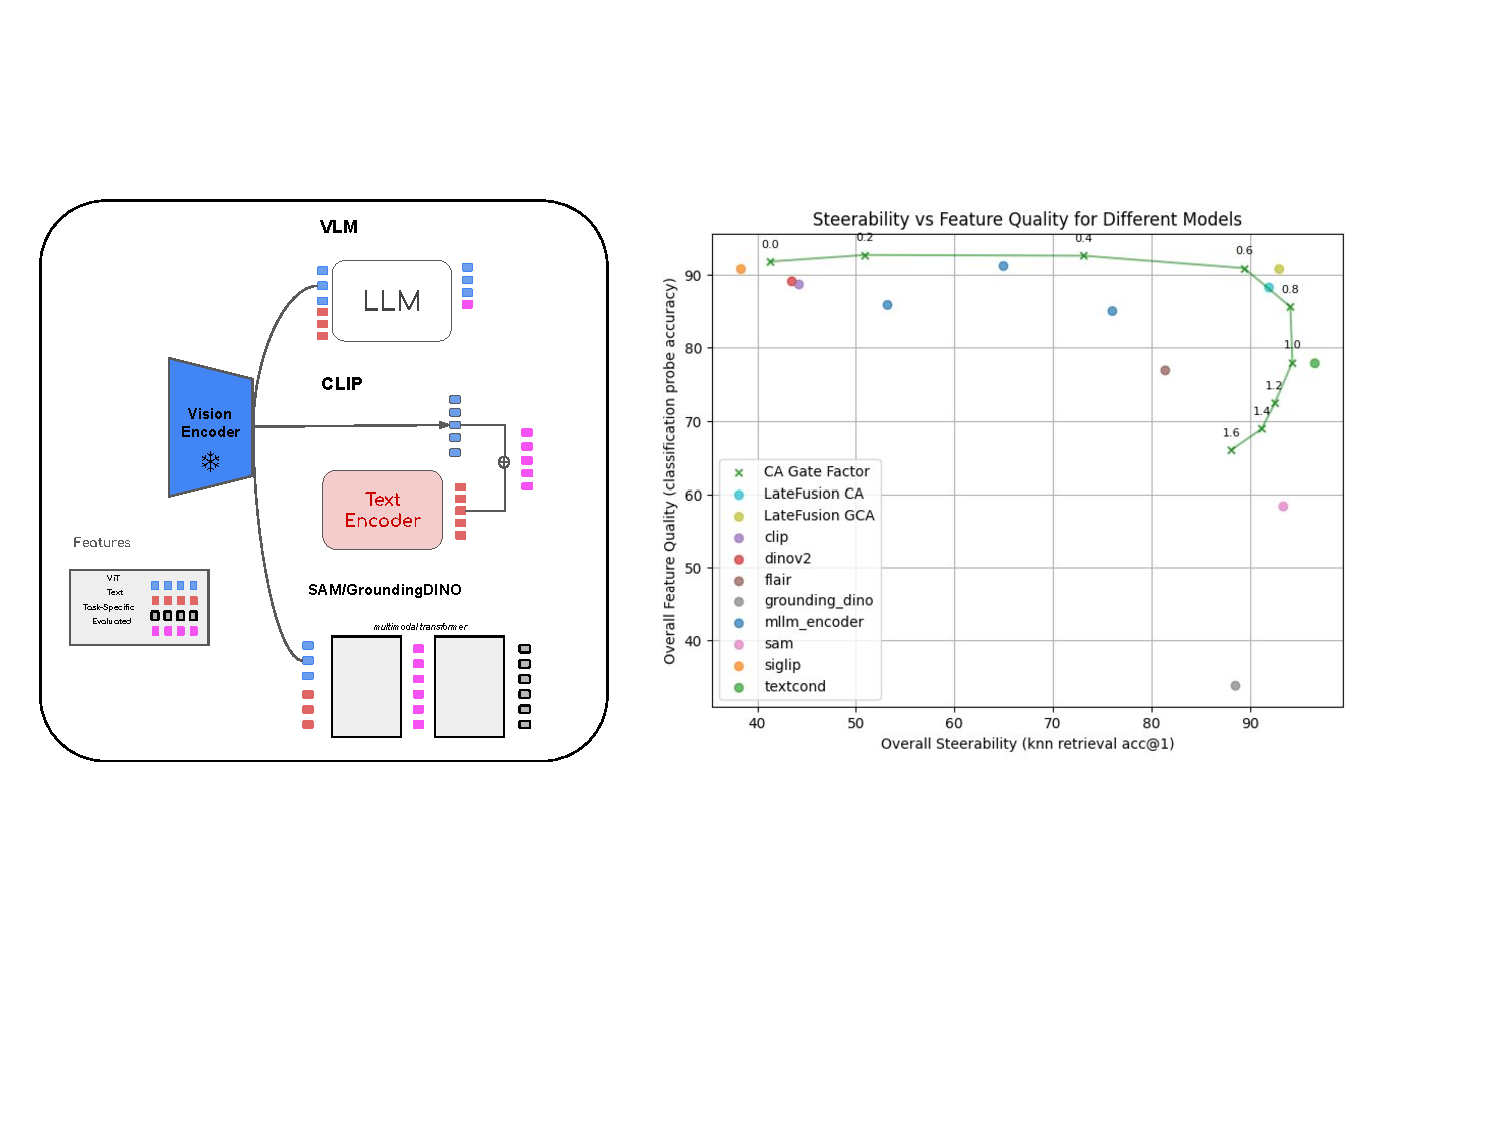
\includegraphics[width=\linewidth]{figures/teaser_3.pdf}
    \caption{\textbf{Top:} Contrasting vision-language representations with our text-conditioned visual representations.
    \textbf{Bottom:} We compare visual features along two axes - quality (global and patch level features on classification and segmentation probes) and text-steerability.
    Standard encoders (DINOv2, SigLIP) produce rich features but cannot be steered.
    Multimodal models (SAM2, GroundingDINO) are steerable but produce task-specific representations that lack generality for downstream transfer.
    SHIFT achieves both high steerability and high feature quality.}
    \label{fig:teaser}
\end{figure}

\section{Introduction}
\label{sec:intro}

Pretrained visual encoders exhibit a strong saliency bias: they effectively process images through the most prominent visual concept in the scene.
This behavior stems from photographer bias in training data, where subjects are centered and in-focus, and paired caption caption used for vision-language modelling typically describe only primary objects.
Self-attention reinforces this tendency by routing global information through high-norm tokens that correspond to salient foreground objects~\cite{caron2021dino, oquab2024dinov2}.
The result is query-agnostic representations that collapse to coarse, scene-level semantics.
Consider a kitchen image containing appliances, utensils, and a few mugs in the background: DINOv2~\cite{oquab2024dinov2} features encode the global ``kitchen,'' scene while discarding the fine-grained concepts needed to retrieve, count, or localize specific objects like the mugs.

This limitation leaves current models trapped between two extremes (Figure~\ref{fig:teaser}).
Standard visual encoders such as DINOv2~\cite{oquab2024dinov2} and SigLIP~\cite{zhai2023_siglip} produce rich, general-purpose features but offer no mechanism to focus on a particular visual concept.
Open-vocabulary localization models such as SAM3~\cite{ravi2024sam2} and GroundingDINO~\cite{liu2023groundingdino} accept text queries but produce task-specific representations that lack the generality and fidelity for downstream transfer.
No existing approach achieves both high-quality visual features and prompt-based steerability.

In this context, we explore the question: \textit{can text conditioning steer the semantics of visual representations without degrading their quality?}
We present SHIFT, a method that equips any frozen Vision Transformer with the ability to steer its features via natural language.
SHIFT interleaves tanh-gated cross-attention layers~\cite{alayrac2022flamingo} within a frozen ViT and trains them on referential segmentation, using the segmentation objective as a proxy signal to learn steerable representations.
We find that this leads to three desirable properties/desiderata:
\begin{itemize}
    \item \textbf{Global steerability:} The text query steers the semantics of the global feature vector, enabling conditional retrieval of non-salient visual concepts (\MG{vague}) in cluttered scenes (Section~\ref{subsec:cond_ret_exp}).
    \item \textbf{Dense attention routing:} Self-attention routes information through tokens corresponding to the text-described visual concept, improving localization for non-salient objects (Section~\ref{subsec:mosaic_exp}).
    \item \textbf{Feature quality preservation:} The steered representations preserve the base ViT's downstream transfer, maintaining \sout{classification and segmentation} performance on standard vision benchmarks (Section~\ref{subsec:pareto}).
\end{itemize}

Together, these properties yield a surprising consequence: text-conditioned steering generalizes to out-of-distribution domains more effectively than supervised fine-tuning.
Because our method preserves the rich visual structure learned from large-scale vision-only pretraining, natural language can focus these features on novel concepts without the catastrophic forgetting that accompanies fine-tuning on limited target data.
On personalized object discrimination, descriptive text prompts outperform a fine-tuned DINOv2 baseline in a zero-shot manner (Section~\ref{subsec:ood_generalization}).
On industrial anomaly detection, a domain entirely absent from training, our general-purpose model matches dedicated methods without any adaptation.

In summary, we make the following contributions:
\begin{enumerate}
    \item We introduce SHIFT, a text-conditioned visual encoder that instills text understanding into frozen ViTs via sparse, gated cross attention layers trained on grounding.
    % sparse, tanh-gated cross-attention layers trained on referential segmentation.
    % \item We demonstrate a Pareto improvement over existing models: SHIFT achieves high text steerability while preserving the feature quality of the underlying ViT, bridging the gap between unsteerable encoders and quality-degraded multimodal models.
    \item We demonstrate a Pareto improvement over existing models:
    % \item Our approach dynamically routes attention to task-relevant visual concepts, 
    SHIFT can guide the semantics of the visual representation with text while preserving their downstream transfer, bridging the gap between unsteerable encoders and quality-degraded multimodal models.
    \item We demonstrate that text conditioning enables zero-shot domain transfer that outperforms supervised fine-tuning: on personalized object discrimination (PODS), descriptive prompts surpass a fine-tuned DINOv2 baseline (54.4 vs.\ 48.0 PR-AUC), and on industrial anomaly detection (MVTec~AD, VisA), our general-purpose model matches dedicated methods, all without task-specific training and across ViT families (DINOv2~\cite{oquab2024dinov2}, SigLIP~\cite{zhai2023_siglip}, MAE~\cite{he2022mae}).
\end{enumerate}

\section{Related Works}
\label{sec:related_work}


% \section{Related Works}

% \begin{itemize}
%     \item Comparing different model families
%     \begin{itemize}
%         \item OV: GroundingDINO, SAM
%         \item MLLMs
%         \item Visual Encoders
%     \end{itemize}
%     \item Text Conditioned Visual Feats
%     \begin{itemize}
%         \item FLAIR
%         \item SAM3 --> MaskInversion
%         \item ELIP, TIE
%     \end{itemize}
% \end{itemize}




\paragraph{Visual Representation Families.}
\JR{in the rest of the paper we use bold text instead of italics for paragraph headings (i.e. subsubsections)}
\YA{technically we should also look at CoCoOp}
Unimodal encoders (DINOv2~\cite{oquab2024dinov2}, MAE~\cite{he2022mae}) learn rich visual representations via self-supervised objectives but produce entirely query-agnostic features.
Cross-modal encoders (CLIP~\cite{radford2021_clip}, SigLIP~\cite{zhai2023_siglip}, CoCoOp~\cite{zhou2022_cocoop}) align image--text embeddings via contrastive or prompt-based pretraining but limit multimodal interaction to post-hoc fusion.
MLLMs achieve moderate steerability by routing visual tokens through a language backbone at substantial computational cost~\cite{chen2025vlm_benchmark}, while open-vocabulary models (GroundingDINO~\cite{liu2023groundingdino}, SAM3~\cite{carion2025_sam3}) are highly steerable but produce localization-specific features that transfer poorly.
We compare these families quantitatively in \cref{tab:method_comparison} and \cref{fig:teaser}.

%%% === Old Visual Representation Families (commented out) ===
% {\color{gray} Modern vision systems extract features through architecturally distinct paradigms.}
% \textit{Unimodal encoders} such as DINOv2~\cite{oquab2024dinov2} and MAE~\cite{he2022mae} learn rich visual representations via self-supervised objectives but produce features that are entirely query-agnostic.
% \textit{Cross-modal encoders} like CLIP~\cite{radford2021_clip} and SigLIP~\cite{zhai2023_siglip} align image and text embeddings through contrastive pretraining, yet their dual-encoder design limits multimodal interaction to post-hoc fusion rather than early feature-level conditioning. 
% \textit{Multimodal large language models} (MLLMs) process interleaved image--text sequences and can produce text-influenced visual representations, but they route visual tokens through a large language backbone, incurring substantial computational overhead for moderate steerability.
% \textit{Open-vocabulary localization models} such as GroundingDINO~\cite{liu2023groundingdino} and SAM3~\cite{carion2025_sam3} fuse text deeply into their encoder through cross-modal attention, yielding highly steerable intermediate features; however, these representations are optimized for localization and transfer poorly to general vision tasks.
% Our work bridges this gap: we condition frozen ViT features on text within the transformer layers themselves, achieving high steerability while preserving the representation quality of the base encoder.
%%% === End old Visual Representation Families ===


\paragraph{Text-Conditioned Visual Features.}
\YA{we should say that this family basically doesn't exist. and highly differentiate/dismiss FLAIR }
% TODO: expand with FLAIR, SAM3/MaskInversion, ELIP, TIE
The goal of producing visual features that are both text-steerable and high-quality remains largely unaddressed.
The closest attempt, FLAIR~\cite{xiao2025flair}, applies text-conditioned attention pooling over frozen CLIP features.
Because this fusion occurs outside the encoder, at the pooling stage, text cannot influence the encoding process itself: FLAIR achieves only moderate steerability and weaker text-dependence (\cref{subsec:cond_ret_exp}), and its features fall short of unimodal encoders on standard vision benchmarks (\cref{fig:teaser}).
Moreover, FLAIR is restricted to CLIP-style backbones and requires two orders of magnitude more training data.
These limitations reflect a deeper asymmetry: high-quality unimodal data---both vision-only and language-only---vastly exceeds paired multimodal data, which is why unimodal encoders learn richer representations in the first place.
This suggests that rather than training joint vision-language encoders from scratch on limited paired data, one should inject language conditioning into strong unimodal vision encoders, preserving the representational depth learned from each modality independently.
The challenge then becomes one of \textit{representation alignment}: how to merge two unimodal experts into an early-fused encoder without degrading either modality's representations.
\model{} addresses this by conditioning a frozen ViT on text within the transformer layers themselves; text serves not as a training signal but as a steering mechanism that preserves the base encoder's quality while extending generalization to domains where labeled data is scarce.

%%% === Old Text-Conditioned Visual Features (commented out) ===
% FLAIR~\cite{xiao2025flair} applies text-conditioned attention pooling over frozen CLIP features to produce text-informed global representations. Unlike \model{}, it operates at the pooling stage rather than within the encoder itself.
% Failure of FLAIR -->
%%% === End old Text-Conditioned Visual Features ===

% SAM3 --> MaskInversion
% ELIP, TIE


\section{\model{}: Steering Vision Transformers with Text}
\label{sec:method}

% method text-conditioned visual
% architecture modifications
% datasets + training signals
% inference-time text conditioning (jona)
% experiments (hypothesis validating) ## arxiv - before method
% conditional retrieval kNN
% baseline: late fusion
% without losing classification
% pareto explain
% attention does steer to text descriptions (results by segmentation)
% analysis / applications
% personalized: how to condition (PODS)
% anomaly detection 
% where are my keys (?)
% (???) hallucination detection, negation 
% (???) VQA
% ablations / features of our approach -- justifying choices of method (a subset of task)
% architecture (sigmoid gating, FFN block, CA blocks)
% backbones (MAE, SigLIP) (?)
% scale the model (ViT-L)
% losses (?)
% resolution (?)
% token length [optional!]
% conclusion

% \MT{skipping for now as discussed with MG}


Next, we describe the architectural modifications and post-training to turn a pretrained ViT into a \model{} model.
% We inject text into a frozen ViT through gated cross-attention layers that steer visual features towards the text prompt without degrading them.
% We describe \model{}'s architectural modifications and training data and objectives below.

% As illustrated in \cref{fig:arch_training}, our architecture consists of three components:
% (1)~a frozen text encoder (RoBERTa-Large~\cite{liu2019roberta}) that produces token-level embeddings from the input prompt;
% (2)~a lightweight multimodal adapter (MLP) that projects these text embeddings into the visual embedding space; and
% (3)~tanh-gated cross-attention layers interleaved within a frozen ViT that progressively fuse textual cues into the visual representation.
% Given an image and a text prompt, SHIFT produces text-contextualized patch-level visual features that remain in the base ViT's embedding space.
% We train the model on a diverse mixture of referential segmentation datasets (Section~\ref{sec:data}) using a binary segmentation objective at the ViT patch level (Section~\ref{sec:objective}).
% The segmentation head serves solely as a training signal and is discarded at inference; the output of interest is the steered visual representation itself.

\subsection{Architecture}
\label{sec:arch}

\begin{wrapfigure}{r}{0.4\textwidth}
\centering
\vspace{-15mm}
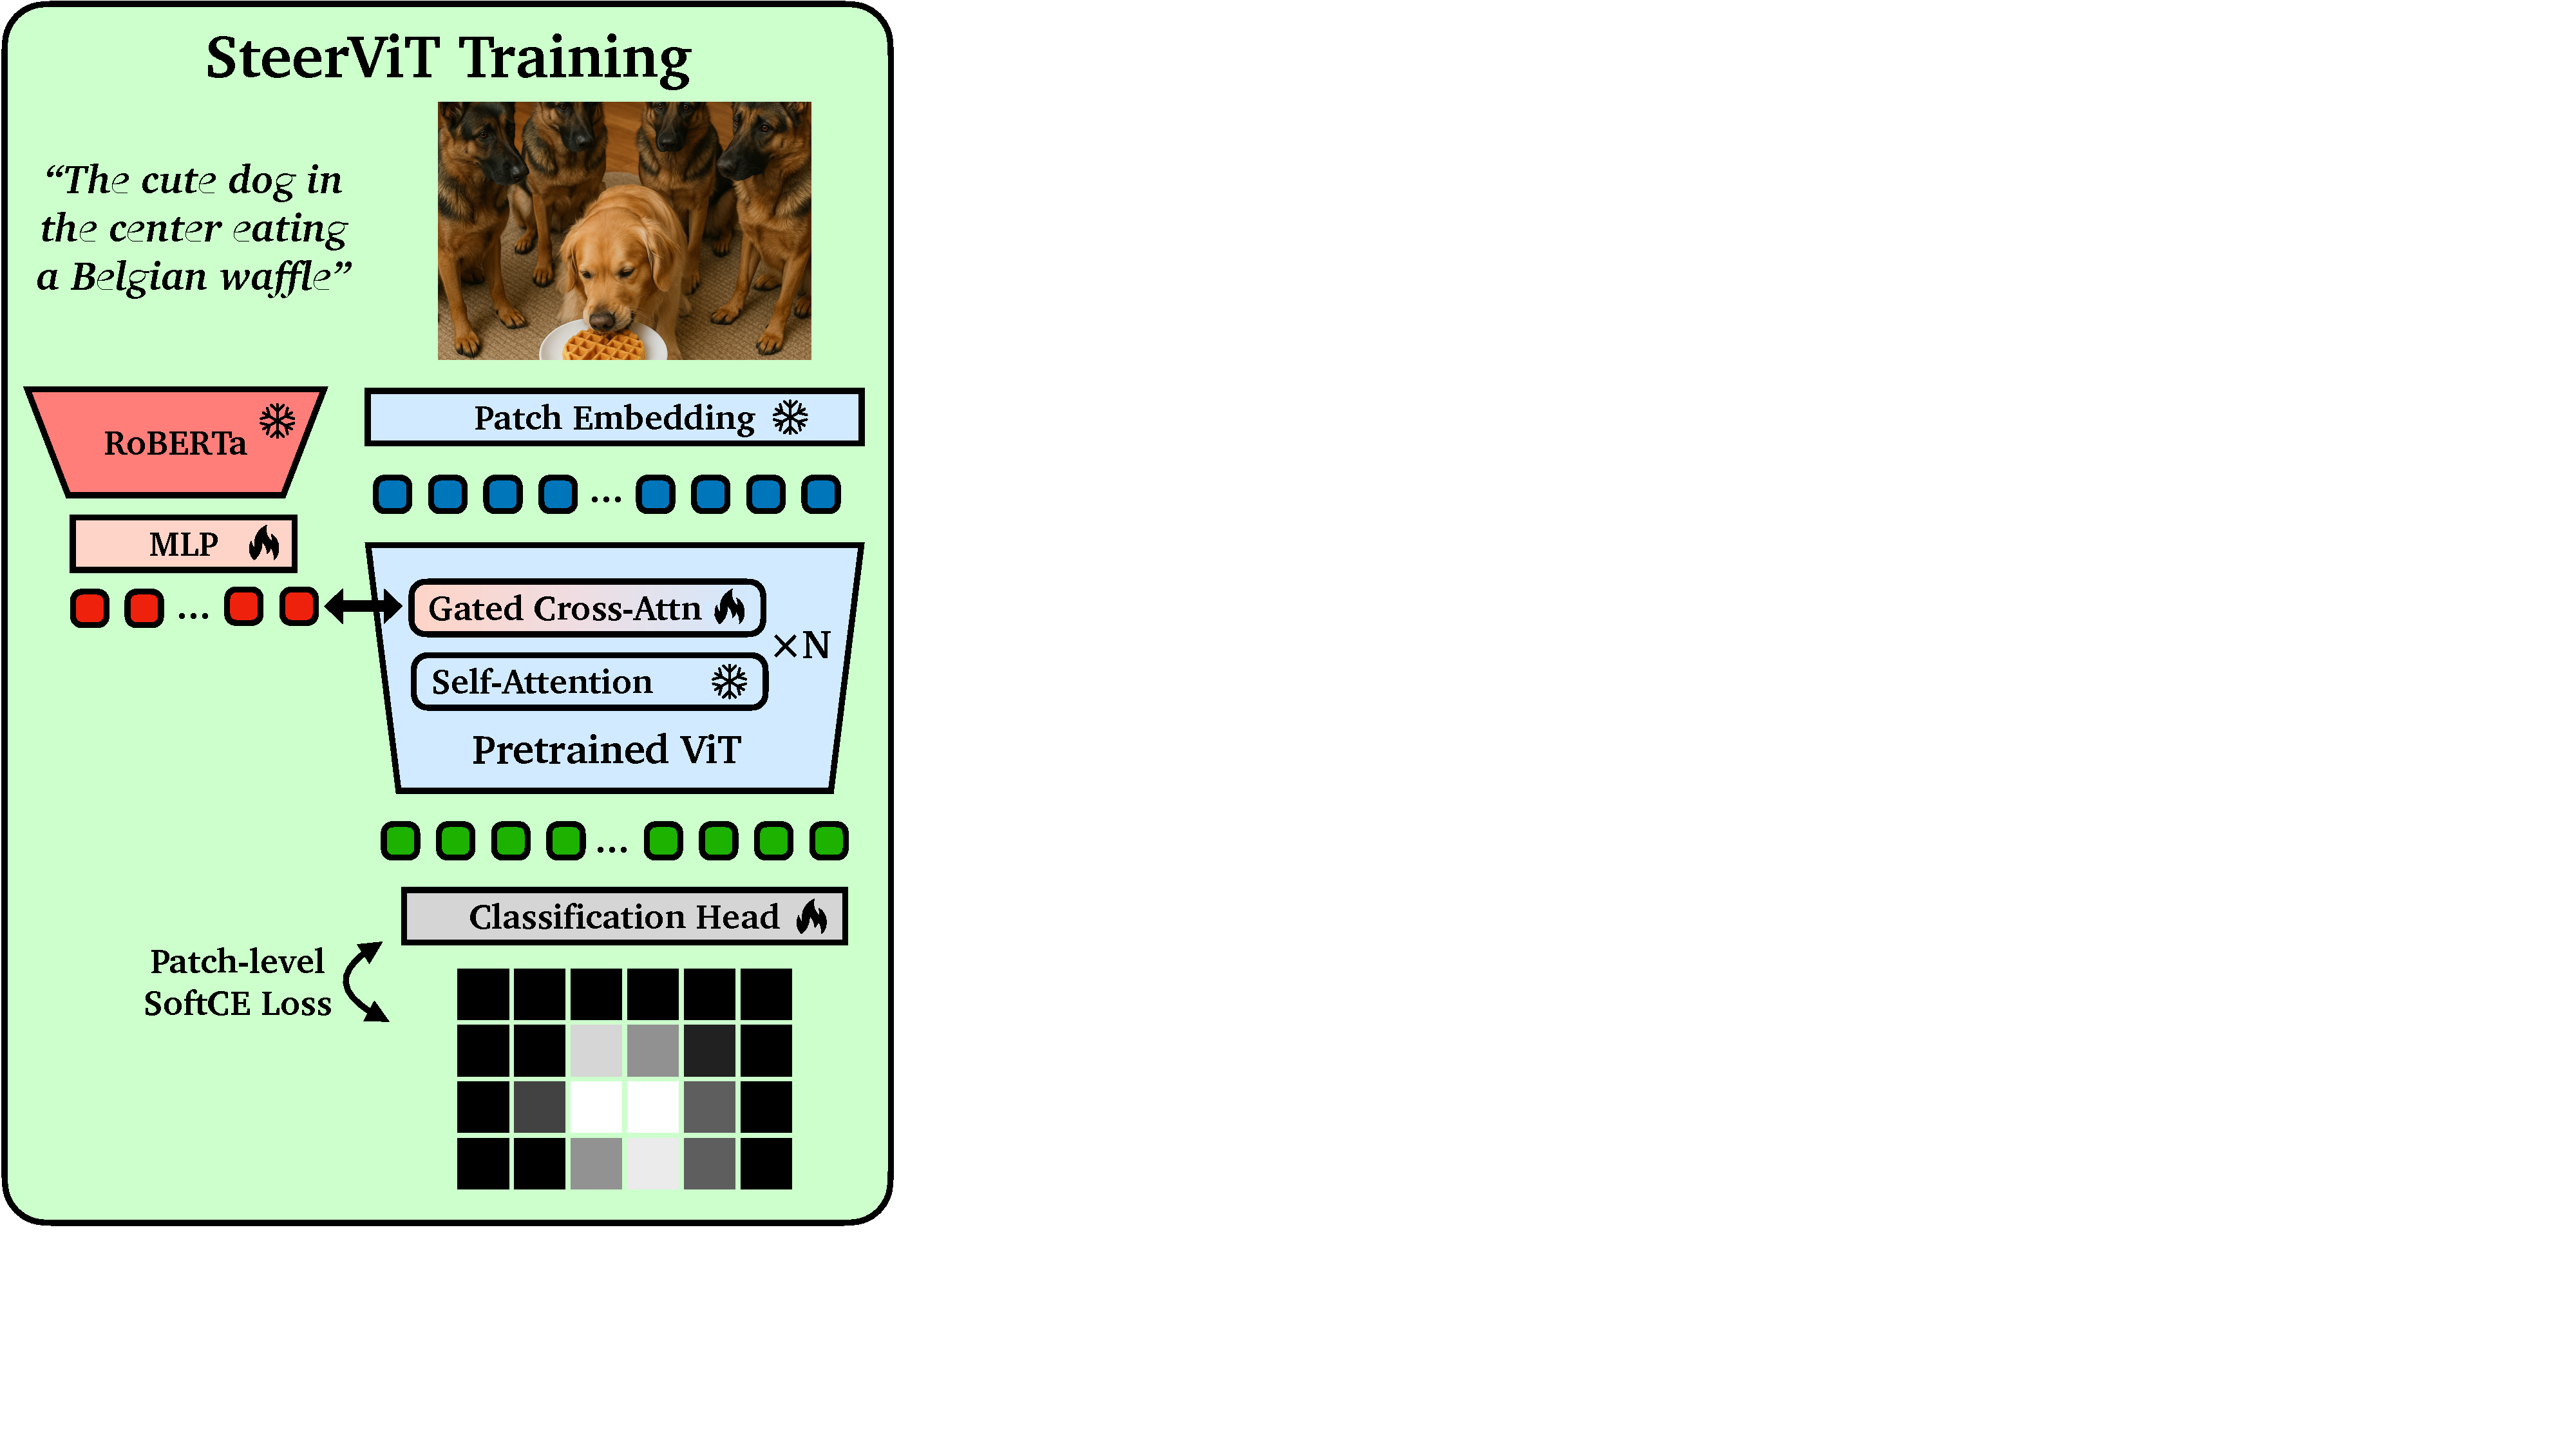
\includegraphics[width=\linewidth]{figures/training_architecture.pdf}
\vspace{-3mm}
\caption{\textbf{Steering any ViT using text conditioning.}
Our method adds lightweight vision-to-language cross-attention layers within pretrained ViT blocks and applies a patch-level segmentation proxy objective to fuse prompt cues into patch tokens. We train on XXXX \YA{add:We train this with existing referential object localisation datasets of X~M images??}
\YA{great job! maybe all RoBERTa-"L"? or "M"? and also add somewhere "pretrained ViT"? }
}
\label{fig:arch_training}
\end{wrapfigure}

As illustrated in \cref{fig:arch_training}, our \model{} consists of four components:

\colorbox{visionblue}{\textbf{A. Visual encoder.}}
For an image $X_v \in \mathbb{R}^{H \times W \times 3}$, a ViT produces a sequence of $N$ patch tokens $Z_v \in \mathbb{R}^{N \times d_v}$ and optionally a  \texttt{[CLS]} token, where $d_v$ is the embedding dimension.
All original ViT parameters remain frozen throughout training; new capacity enters exclusively through the interleaved cross-attention layers described below.
While most experiments adopt the DINOv2 ViT-B/14~\cite{oquab2024dinov2} as our backbone, we will show that our approach also improves steerability of SigLIP or MAE.


\colorbox[RGB]{234,133,125}{\textbf{B. Text encoder.}}
We adopt a frozen, pretrained text encoder (RoBERTa-Large~\cite{liu2019roberta}) to produce token-level embeddings $Z_t \in \mathbb{R}^{L \times d_t}$ for a given input conditioning prompt $X_t$, where $L$ is a variable number of text tokens and $d_t$ is the text embedding dimension.
% Given an input prompt $X_t$, the encoder extracts a variable-length sequence of token embeddings $Z_t \in \mathbb{R}^{L \times d_t}$, where $L$ is the number of text tokens and $d_t$ is the text embedding dimension.
% We $\ell_2$-normalize these embeddings before passing them to the multimodal adapter.

\colorbox{textred}{\textbf{C. Multimodal adapter.}}
Each language embedding $Z_t^i$ is $\ell_2$-normalized and fed through a trainable two-layer MLP that projects the sequence into visual-aligned tokens $H_t \in \mathbb{R}^{L \times d_v}$.
We add learnable positional encoding to $H_t$ to preserve token order before injecting them into the ViT through the gated cross-attention mechanism. 
\YA{I think it wouldn't hurt to describe the steps you're doing with math.. including actually the L2 normalisation earlier etc. }



\tikz[baseline=(X.base)] 
\node[rectangle,
      inner sep=2pt,
      outer sep=0pt,
      shade,
      left color=textred,
      right color=visionblue] (X)
{\textbf{D. Gated cross-attention layers.}}; % <-- DON'T remove - Semicolon needed to tikz to compile without error
To fuse textual conditioning into the ViT's residual stream, we invert the gated cross-attention (CA) formulation from Flamingo~\cite{alayrac2022flamingo} by allowing hidden vision states to attend to language tokens (language-to-vision CA in \cite{alayrac2022flamingo}).
We insert CA layers into every other Transformer encoder block (e.g., 6 CA layers across 12 blocks in ViT-B), with each layer consisting of multi-head cross-attention followed by a feed-forward network (FFN).
% To fuse textual conditioning into the ViT's residual stream, we adapt the gated cross-attention (CA) dense formulation from Flamingo~\cite{alayrac2022flamingo} \YA{, but essentially apply it in a reverse manner: we let the vision model look at text-features, not the other way around. (something like this)}.
% Each inserted layer applies multi-head cross-attention followed by a feed-forward network (FFN).
The visual patch tokens $Z_v^{(\ell)}$ at layer $\ell$ serve as queries and the adapted text tokens $H_t$ serve as keys and values:
\begin{equation}
\small
\hat{Z}_v^{(\ell)} = \text{CA}(Z_v^{(\ell)}, H_t) = \text{softmax}\!\left(\frac{Q K^\top}{\sqrt{d_k}}\right) V, \quad Q = Z_v^{(\ell)} W_Q, \; K = H_t W_K, \; V = H_t W_V \, .
\end{equation}
The output is integrated into the residual stream through a tanh gate with a layer-specific learnable scalar $\alpha_\ell$, initialized to zero:
\begin{equation}
Z_v^{(\ell+1)} = Z_v^{(\ell)} + \tanh(\alpha_\ell) \cdot \text{FFN}\!\left(\hat{Z}_v^{(\ell)}\right).
\label{eq:gated_ca}
\end{equation}
Since $\tanh(0) = 0$, the model is mathematically identical to the frozen ViT at initialization.
% As training progresses, the gates learn to open, allowing the model to smoothly incorporate text conditioning. 
Despite the zero-initialisation, the gate still receives a learning signal since
\begin{equation}
\frac{\partial Z_v^{(\ell+1)}}{\partial \alpha_\ell}
=
\mathrm{sech}^2(\alpha_\ell)\,\mathrm{FFN}\!\left(\hat{Z}_v^{(\ell)}\right),
\end{equation}
and $\mathrm{sech}^2(0)=1$. %, yielding \( \left.\frac{\partial Z_v^{(\ell+1)}}{\partial\alpha_\ell}\right|_{\alpha_\ell=0} = \mathrm{FFN}(\hat{Z}_v^{(\ell)}).\)
Thus, $\alpha_\ell$ can move away from zero during optimization, gradually activating the conditioning pathway and allowing the model to incorporate language-based clues.

\subsection{Training Objective}
\label{sec:objective}
In order to encourage the vision encoder to leverage and incorporate language clues, we design a pretext task requiring consideration of the prompt to be solved. We select referential segmentation for this purpose, where, given an image $X_v$ and a prompt $X_t$ referring to a target object, the model predicts which patches correspond to the referred object.


The ground-truth is given by the fraction of foreground pixels within of a pixel-wise binary segmentation mask that was patchified to match the ViT's $n \times n$ grid of non-overlapping patches.
% The ViT partitions the image into an 
% We convert the ground-truth binary segmentation mask $M \in \{0, 1\}^{H \times W}$ into patch-level labels $y \in [0, 1]^{n \times n}$ by computing the fraction of foreground pixels within each patch.
A linear classifier head maps each patch representation $Z_v^i \in \mathbb{R}^{d}$ to a probability $p_i$ through softmax.
We adopt the soft cross-entropy loss
\begin{equation}
\mathcal{L} = - \sum_{i=1}^{n \times n} y_i \log p_i \, ,
\label{eq:loss}
\end{equation}
% We optimize the network with a binary cross-entropy loss over all patches:
% \begin{equation}
% \mathcal{L} = -\frac{1}{n^2} \sum_{i=1}^{n^2} \left[ \hat{y}_i \log \sigma(p_i) + (1 - \hat{y}_i) \log (1 - \sigma(p_i)) \right],
% \label{eq:loss}
% \end{equation}
% where $\sigma$ denotes the sigmoid function.
as it encourages the CA layers to route
% task-relevant
textual information into the corresponding visual patch tokens, producing steered representations.
% as a byproduct.
Performing segmentation on a patch- rather than pixel-level reduces the training complexity and forgoes the need for pixel-level decoders. 


\subsection{Training Data}
\label{sec:data}

We train on a mixture of referential segmentation and grounding datasets to ensure diversity in both visual domains and textual expression styles:

\textbf{RefCOCO, RefCOCO+, RefCOCOg}~\cite{kazemzadeh2014referitgame, yu2016refcocog} provide referring expressions grounded in COCO images.
RefCOCO+ excludes spatial language (e.g., ``left of''), encouraging the model to rely on appearance cues, while RefCOCOg contains longer, more descriptive expressions that exercise the model's capacity for detailed textual understanding.

\textbf{Visual Genome}~\cite{krishna2017visual} (preprocessed following MDeTr~\cite{kamath2021mdetr}) contributes region descriptions paired with bounding boxes across densely annotated scenes.
These descriptions span a broader vocabulary and more complex spatial relationships than the RefCOCO family, increasing the diversity of text conditioning signals.
We use SAM2 to convert bounding boxes to binary segmentation masks.

\textbf{Mapillary Vistas}~\cite{neuhold2017mapillary} provides street-level imagery with fine-grained panoptic annotations.
Including this dataset expands the visual domain beyond COCO's indoor and object-centric bias toward outdoor, driving, and urban scenes, improving out-of-distribution generalization. We use Describe Anything's synthetically generated referential expressions along with accompanying binary segmentation masks. 

This combination \YA{overall X million images and Y annotations} exposes the model to varied scene complexities (from single objects to dense urban panoramas), expression lengths (from two-word labels to multi-sentence descriptions), and visual domains (indoor, outdoor, street-level), encouraging robust text-conditioned representations.
\YA{in expeirments, you should describe training batch size, iterations count, resolution, GPU hours}

\YA{I think we need one more subsection in Section 3 about "Measuring Text-steerability of vision representations" where we describe the task/benchmarks}
\section{Experiments}


% method text-conditioned visual
% architecture modifications
% datasets + training signals
% inference-time text conditioning (jona)
% experiments (hypothesis validating) ## arxiv - before method
% conditional retrieval kNN
% baseline: late fusion
% without losing classification
% pareto explain
% attention does steer to text descriptions (results by segmentation)
% analysis / applications
% personalized: how to condition (PODS)
% anomaly detection
% where are my keys (?)
% (???) hallucination detection, negation 
% (???) VQA
% ablations / features of our approach -- justifying choices of method (a subset of task)
% architecture (sigmoid gating, FFN block, CA blocks)
% backbones (MAE, SigLIP) (?)
% scale the model (ViT-L)
% losses (?)
% resolution (?)
% token length [optional!]
% conclusion

In this section, we empirically validate properties of our learned steerable representations and show applications to diverse tasks such as personalized object discrimination or anomaly detection.


\subsection{Baselines}
\label{subsec:baselines}

% We benchmark \model{} against a number of existing methods that allow for prompt-based steering of their internal visual representations as well as unimodal vision encoders.

We compare \model{} against baselines spanning multiple model families that differ in how, and whether, they incorporate text into visual features (see 
% \cref{sec:related_work} for an extended discussion and 
\cref{app:baseline_extraction} for feature-extraction details):
% \begin{enumerate}[label=(\roman*),nosep]
% \item 
(1)~\textbf{Unimodal vision encoders}: DINOv2~\cite{oquab2024dinov2} and MAE~\cite{he2022mae}, produce query-agnostic features with no text conditioning.
% \item 
(2)~\textbf{Cross-modal encoders}: CLIP~\cite{radford2021_clip} and SigLIP~\cite{zhai2023_siglip}; we fuse visual and text embeddings via post-hoc element-wise addition (late fusion).
% \item \textbf{FLAIR}~\cite{xiao2025flair}: A cross-model encoder that applies learned text-guided attention pooling over frozen visual features.
% \item
(3)~\textbf{MLLMs}: InternVL3-1B and InternVL3-2B, from which we extract text-contextualized visual features via the last language-block's image-token states.
\MT{slack says E5-V ..}
\MT{see comment of text/image tokens order on slack}
\MT{also mention Qwen3VL-2B, we have results on that, can say InternVL3 and Qwen3VL families}
% \item
(4)~\textbf{Open-vocabulary (OV) localization}: SAM3~\cite{carion2025_sam3} and GroundingDINO~\cite{liu2023groundingdino}; we evaluate the 
% modality-fused encoder state
intermediate multimodal state as text-steered visual representations.
% \end{enumerate}


Where supported, all models process images at $336\times336$ resolution; for models with fixed input dimensions, we resize to this resolution.
% to ensure comparable visual information.


% For \textbf{cross-modal encoders} (e.g., CLIP~\cite{radford2021_clip}, SigLIP~\cite{zhai2023_siglip}, dino.txt), images and prompts are embedded independently using their respective encoders, limiting multimodal interaction to a simple post-hoc late-fusion, where the resulting visual and text features are combined via element-wise addition. 
% As with the considered \textbf{vision-only baselines}, global feature aggregation is conducted as intended by the base method (e.g., CLS or mean pooling). 
% FLAIR~\cite{xiao2025flair} is a CLIP-style model that is trained to produce text informed visual features by applying text-conditioned attention pooling on top frozen visual features.
% % FLAIR~\cite{xiao2025flair} is a CLIP-style model that is specifically trained to produce text informed visual features by applying text-conditioned attention pooling on top frozen visual features tokens.
% We extract text contextualized visual features from \textbf{MLLMs} by concatenating the user prompt $t$ followed by the image $I$ into a multimodal input sequence and selecting the last-language-block states at image-token positions. 
% For global features, we adapt the last-token pooling approach of E5-V~\cite{Jiang2024E5VUE} and append a postfix instructing the model to summarize the image contents in one word while focusing on the aspect specified by $t$.

% Text-conditioned representations are obtained from \textbf{open-vocabulary localization methods} via the modality-fused encoder states, ignoring decoder components responsible for generating bounding boxes or segmentation mask. 
% Specifically, with SAM3~\cite{carion2025_sam3}, we take the patch-level outputs of the \textit{Fusion Encoder} and apply mean-pooling to get image-level features. 
% Similarly, we use the outputs of the cross-modal \textit{Feature Enhancer} layer of GroundingDINO~\cite{liu2023groundingdino}. However, as features are available across multiple spatial scales, we first interpolate them to a common intermediate feature scale before being averaged to get dense pseudo-patch-level features. 
% % \todo{ensure consistency with Methodology Section}

% Where supported by the underlying architecture, we process images at a resolution of $336\times336$. For models with non-configurable input dimensions, we still resize to this resolution prior to processing to ensure comparable levels of visual information.


\subsection{COnditional REtrieval: Steering Global Semantics with Text}


\label{subsec:cond_ret_exp}
\begin{figure}[h!]
\centering
% Left Figure: UMAP
\begin{subfigure}[b]{0.4\textwidth}
\centering
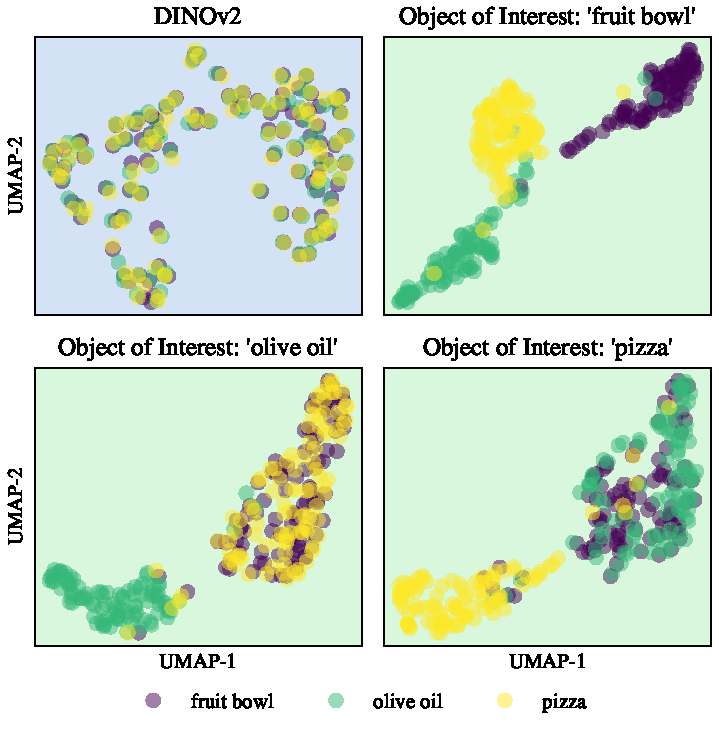
\includegraphics[width=\textwidth]{figures/core_qualitative_objects_scatter.pdf}
\caption{
Feature distribution across three object types  in ``kitchen'' scene.
% DINOv2 embeddings are show no separability across inpainted objects, whereas our text-conditioned embeddings form distinct clusters for each queried concept.
}
\label{fig:umap-neighbourhood}
\end{subfigure}
\hfill
% Right Figure: DinoV2
\begin{subfigure}[b]{0.59\textwidth}
\centering
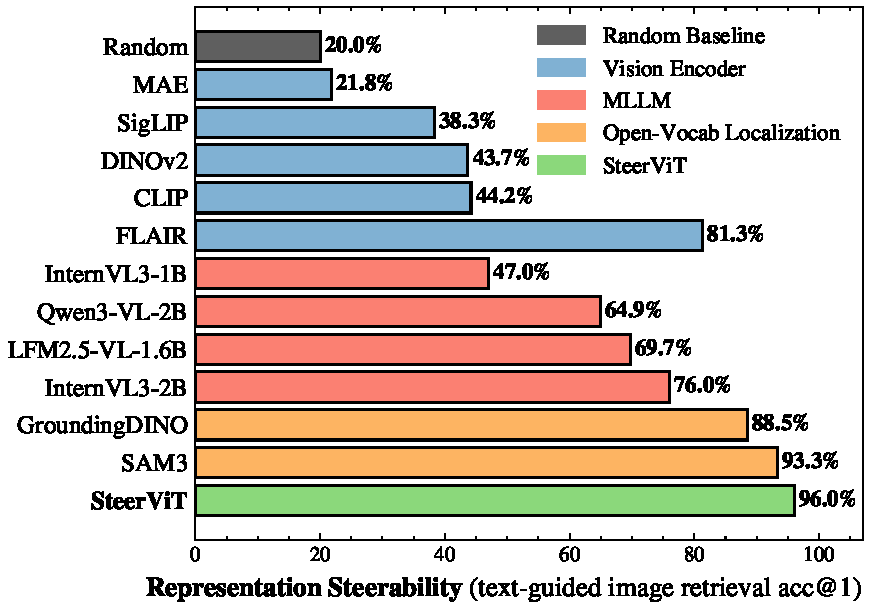
\includegraphics[width=\textwidth]{figures/steerability_bar_chart.pdf}
\caption{
Non-salient object retrieval performance on CORE across model families. 
% Query-agnostic encoders collapse to scene-level semantics and fail conditional retrieval.
% Our method steers global features with text, achieving 93.4\% retrieval accuracy.
}
\label{fig:cond_ret_bar}
\end{subfigure}
\caption{\textbf{COnditional REtrieval (CORE) benchmark.} \textbf{Left:} While DINOv2 features form scene-level clusters, appropriate prompting of \model{} yields object-specific clusters. \textbf{Right:} Substantial differences in steerability between model families exist, with OV localization methods and \model{} offering the greatest adaptability. 
}
\label{fig:cond_ret_baselines}
\end{figure}

% \begin{figure}[h!]
%   \centering
%   
\includegraphics[width=0.98\textwidth]{old_figures/cond_retrieval_baselines.png}
%   \caption{
%   \textbf{Evaluating Vision Steerability of different model families}. Comparison of our method against 
%   }
%   \label{fig:cond_ret_baselines}
% \end{figure}

To measure the degree to which text prompts can actively steer the global image representations, we propose a text-conditional retrieval benchmark, dubbed CORE (COnditional REtrieval).

We select 100 images for each of \MT{3 indoor, 3 outdoor?}
six indoor and outdoor scenes from the SUN397 dataset~\cite{Herranz2016_SUNdataset} and inpaint five scene-relevant peripheral objects into every image using the FLUX.2 image editing model \cite{flux-2-2025}
(e.g., a fruit bowl in a kitchen; a backpack in the park)\footnote{See Appendix \ref{} \JR{TODO} for details and qualitative examples.}.
\MT{same object? how is same object appropriate across all scenes?}
By framing the problem as one-vs-all retrieval where, given a query image with inpainted object $\Omega$, the objective is to retrieve other instances containing $\Omega$ within a scene $\text{S}$ (e.g., ``fruit bowl'' in ``kitchen''), we can quantify how well models prioritize specified non-salient background objects over scene-level visual similarities in their global representations.
\MT{too long sentence, splitting and shortening:
We frame the problem as one-vs-all retrieval---given a query image with inpainted object $\Omega$, the goal is to retrieve other instances containing $\Omega$ within a scene $\text{S}$.
CORE allows us to quantify how well models prioritize specified non-salient background objects over scene-level visual similarities in their global representations.
}
Here, both the query as well as the gallery images are extracted by conditioning on the name of the query object $\Omega$.
%(e.g., ``the fruit bowl'').% to prevent ground-truth leakage through the text embeddings. 
We measure the top-1 retrieval accuracy over the remaining 495 non-identical instances in $\text{S}$ and average over objects.
% The random chance is 20\%, since 99 out of 495 candidates share the query object.


\subsubsection{Query-agnostic encoders collapse to salient concepts.}

\MT{usually not capitalized, sentence case}
Query-agnostic encoders fail at conditional retrieval because their features collapse to the dominant scene concept (Figure~\ref{fig:cond_ret_baselines}).
MAE barely exceeds random chance; DINOv2, despite its object-centric representations, achieves only 43\% R@1 
% \MT{retrieval accuracy @ 1}.
Cross-modal visual encoders (CLIP, SigLIP) also perform poorly without text conditioning despite operating in a shared vision-language space.
In contrast, \model{} achieves 94.3\% retrieval accuracy, confirming that text conditioning shifts the global representation from the scene level (``kitchen'') to the queried concept (``fruit bowl'').
% Among unimodal encoders, MAE barely exceeds random chance while DINOv2 roughly doubles MAE's accuracy owing to its more object-centric representations but only achieves 43\%.
% Even multimodal encoders (CLIP, SigLIP) fail: post-hoc late fusion with text cannot rescue features that were never conditioned on the query.
% Our method on the other hand achieves 94.3\% retrieval accuracy (cf., Figure~\ref{fig:cond_ret_baselines}), confirming that text conditioning shifts the global representation from the scene level (``kitchen'') to an object-of-interest-specific/prompt-steerable representation \MG{consistent with Fig2a} (``fruit bowl'').
% Query-agnostic encoders fail at conditional retrieval because their features collapse to the dominant scene concept (Figure~\ref{fig:cond_ret_baselines}).
% MAE barely exceeds random chance, and DINOv2 roughly doubles MAE's accuracy owing to its more object-centric representations.
% CLIP and SigLIP, despite operating in a multimodal embedding space, are unable to contextualize their visual features through post-hoc late fusion with text.
% In contrast, our method achieves 96.6\% and 91.3\% accuracy on indoor and outdoor scenes respectively, confirming that text conditioning shifts the global representation from the scene level (``kitchen'') to the queried concept (``mug in kitchen'').
% an unconditional feature improvement.

Figure~\ref{fig:umap-neighbourhood} illustrates this on ``kitchen'' scenes via UMAP.
DINOv2 embeddings (left) show no separability across inpainted object types,
% DINOv2 embeddings show no separability across inpainted object types, 
whereas our text-conditioned embeddings form distinct clusters for different text prompts.
This confirms that \model{} can reorganize its embedding space around the queried concept.
% When conditioned on ``fruit bowl'' (right), our method produces three distinct groups: a tight cluster of fruit-bowl instances, a secondary group of semantically related kitchen objects, and remaining unrelated objects pushed to the periphery, confirming that text conditioning reorganizes the embedding space around the queried concept.
% Figure~\ref{fig:umap-neighbourhood} illustrates this in ``kitchen '' scenes via UMAP: DINOv2 embeddings show no separability across inpainted object types, whereas our text-conditioned embeddings form distinct clusters for each queried concept.
% \MT{please describe how to interpret fig 2a better; describe how fire hydrant also pulls basketball?}


% \subsubsection{CLIP/SigLIP's Text Encoder Do Not Enable Steerability}
\subsubsection{Post-hoc late fusion does not enable steerability.}
A natural follow-up is whether post-hoc fusion with text can rescue query-agnostic ViTs?
We explore this for CLIP and SigLIP, which share a multimodal embedding space by fusing visual features with text embeddings via element-wise addition.
This yields a negligible 0.02\% boost, confirming that post-hoc late fusion cannot steer frozen representations.
Early fusion within the ViT layers is essential: \model{}, which conditions intermediate representations on text via cross-attention, improves retrieval accuracy from below 43\% to 94.3\%.
% A natural follow-up is whether post-hoc fusion with text can rescue query-agnostic representations.
% For CLIP and SigLIP,which already share a multimodal embedding space, we fuse visual features with text embeddings via element-wise addition.
% This yields a negligible boost of 0.02\%, confirming that late fusion cannot steer query-agnostic frozen representations. 
% Learning query-aware features within the ViT layers (early fusion) is essential.
% \MG{dino.txt - same results; post-hoc late fusion doesn't work}
% \MG{contrast with random conditioning}
% \MG{contrast with FLAIR/MaskInversion}
% A more comparable study for late fusion would be add the cross attention layer on top of the frozen ViT features. We find that this although enables steerability, the downstream performance of the multimodal features are suboptimal for fine-grained vision-lanuage tasks. We discuss it in detail in Section~\ref{sec:method}. # dont delete comment
FLAIR~\cite{xiao2025flair} tries to bridge cross-modal encoders with text-steerable features by training text-conditioned attention pooling over frozen ViT features.
This achieves steerability (81.3\%) but still significantly lags \model{} by 13\%.
Moreover, unlike \model{} which adapts any frozen ViT family, FLAIR is restricted to CLIP-style backbones and requires two orders of magnitude more training data.
% \textbf{FLAIR} tries to bridge CLIP/SigLIP style models with text steerable encoders by training text-informed attention pooling over query-agnostic ViT features. This enables text steering but still lags behind our method (by 13\%). Moreover our method is agnostic to visual encoder family, however FLAIR is a cross-modal encoder. They require 2 orders of magnitude larger data, while we can efficient adapt any ViT to be text-steerable.

\newif\iffindingbox
\findingboxtrue
\iffindingbox
\begin{tcolorbox}[colback=lightyellow,
colframe=black, arc=4pt, boxsep=1pt]
\paragraph{\textbf{\textit{Finding} 1.}}
Our method can steer the semantics of the visual features with text while standard vision encoders collapse to the loudest concept in the image.
\MT{shouldn't this come at the end of this section?}
\end{tcolorbox}
\fi

% \subsubsection{Steerable but inefficient or specialized: MLLMs and OV models.}
\subsubsection{MLLMs and OV models are steerable, but inefficient or specialized.}

\textit{MLLMs} can moderately steer visual features but at substantial computational cost.
InternVL3-1B scores only 51.2\%; scaling to 2B raises this to 77\%. \MT{76?}
\model{} outperforms both variants by 40\% and 14\% \MT{16?} respectively while adding only 130M parameters via cross-attention blocks. \MG{Add FLOPs}
Open-vocabulary localization models (GroundingDINO, SAM3) on the other hand are highly steerable, with SAM3 nearly matching \model{}'s retrieval accuracy.
However, their intermediate representations are optimized for localization and lack the generality needed for downstream transfer, as we discuss in \cref{subsec:pareto}.

% \subsubsection{MLLMs: Steerable but Inefficient}
% MLLMs can moderately steer visual features, but at substantial computational cost.
% InternVL3-1B scores only 51.2\%; scaling the LLM to 2B parameters raises this to 77\%.
% Our method
% outperforms their 1B and 2B variants by 40\% and 14\% respectively while adding only 130M parameters to visual encoder via cross-attention blocks. \MG{Add FLOPs}
% In fact, our approach can be viewed as an inverted MLLM: instead of conditioning a language model on frozen visual features (late fusion), we condition the visual features on text within the ViT layers themselves (early fusion).
% Recent work~\cite{chen2025vlm_benchmark} finds that that VLMs perform substantially worse than their underlying visual encoder on vision-centric benchmarks.
% Because the text directly influences visual representation learning process, SteerViT can guide attention toward task-relevant regions in a way that post-hoc fusion cannot.
% \MG{(out-of-place)}
% \subsubsection{Open-Vocabulary (OV) Localization}
% GroundingDINO and SAM3 are highly steerable, with SAM3 nearly matching \model{}'s retrieval accuracy.
% They apply heavy multimodal processing on their visual backbones for task-specific optimization.
% However, although features extracted from them are steerable with text, these features are task-specific i.e localization. As illustrated in Figure~\ref{fig:teaser}, these features are transferrable for downstream reuse, scoring poorly on standard vision benchmarks. Unlike our method,     preserves the representation quality of the visual encoder. We discuss this further in Section~\ref{}. #dont delete comment
% However, their intermediate representations are optimized for localization and lack the generality needed for downstream transfer, as we analyze in Section~\ref{subsec:pareto}.

\subsubsection{Conditioning on a random class breaks retrieval.}

% \MT{title is not a finding unlike others above; a simple modification: Conditioning on a random class breaks retrieval.}
To verify that steerability is genuinely text-driven rather than an artifact of training, we condition each model on a random (incorrect) object class and measure the retrieval degradation (hatched bars in Figure~\ref{fig:cond_ret_baselines}).
\MT{guys, this is removed! discuss without the figure?}
CLIP and SigLIP show no degradation under random conditioning, confirming their features are unconditionally visual and not steerable.
FLAIR exhibits a moderate drop ($-36.1\%$), while \model{} drops by $-50.8\%$, indicating stronger text-dependence.
\MG{these are relative\%}
OV models also see large drops, consistent with their deep text integration.
MLLMs show only mild sensitivity, with InternVL3-1B declining by $-16.1\%$.
\model{}'s catastrophic degradation under random conditioning confirms that its steerability is driven by the text query rather than by the training objective or data.

% CLIP,SigLIP post hoc late fusion - no performance degradation when conditioning on random object class. multimodal feature not steerable with text. feature is unconditional visual
% FLAIR - random conditioning doesn't decrease performance as much ours (-36.1\% v/s -50.8\% for ours), early fusion remains more steerable.
% OV methods see big dip, very steerable. MLLMs not as much, very slight dip for MLLMs, especially if small i.e internvl3-1b sees only -16.1\% decrease
% our method - conditioning on a random object class instead of the correct one causes retrieval performance to degrade catastrophically, demonstrating that the steerability is indeed driven by the text query rather than by fine-tuning data or objective.


In summary, only \model{} and OV localization models are text-steerable,
standard ViTs collapse to salient concepts, 
post-hoc late fusion fails for CLIP-style models, and
although MLLMs offer moderate steerability, it comes at a prohibitive cost.

% In summary, our method and open-vocabulary localization models (SAM3, GroundingDINO) can steer global semantics with natural language, whereas standard vision encoders collapse to salient objects.
% MLLMs exhibit moderate steerability but remain parameter-inefficient.

% Table: kNN experiments

\subsection{MOSAIC Localization: Text enables Targeted Attention \sout{Routing}}
\label{subsec:mosaic_exp}
% \subsection{Steering Attention}


\begin{figure}[t]
\centering
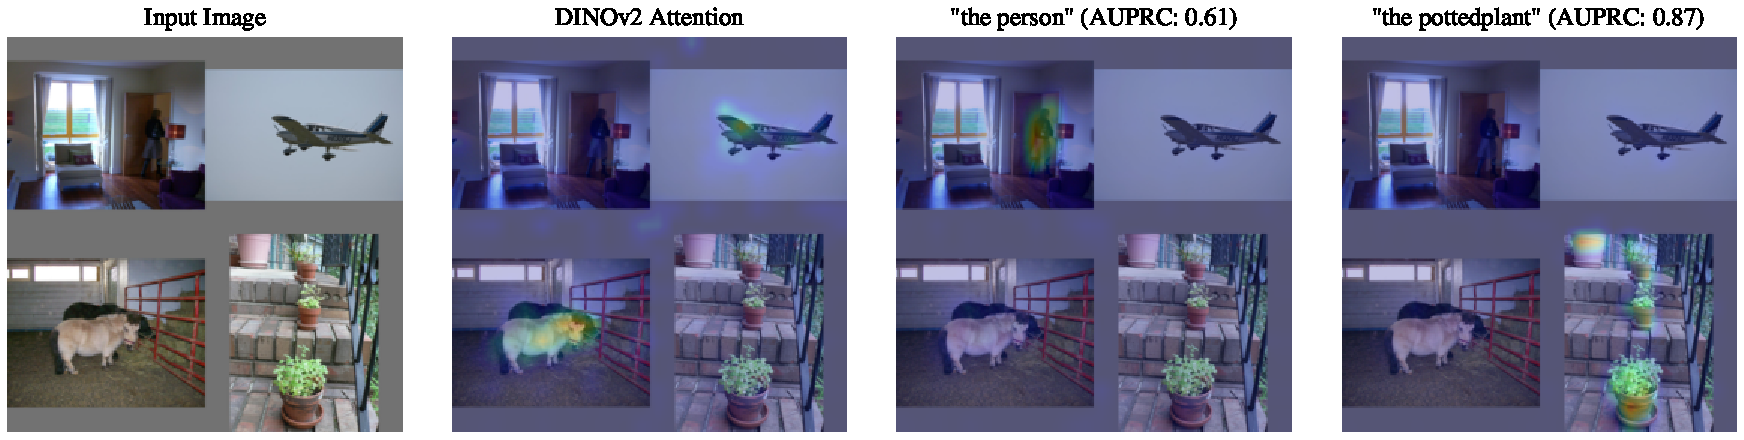
\includegraphics[width=\textwidth]{figures/mosaic_attention_maps.pdf}
\vspace{-2mm}
\caption{\textbf{Text routes dense attention.} Attention maps on a four-image mosaic demonstrate that text conditioning redirects self-attention from salient objects to the queried concept whereas DINOv2 attends to the most prominent objects (``pony'' and ``airplane'').
\JR{heatmap overlay is not properly exported to PDF; needs fixing}
\YA{need to say/show that last two panels are w/ SteerViT}}
\label{fig:steer_attn}
\end{figure}

% \MT{do we want to highlight task or takeaway in subsec headers? benchmarks are new, so ok to focus on takeaways here}
% \MG{Not sure} \JR{since we do it later, would make sense to also do it here for the subsubsecs}

% In the previous section, 
We demonstrated that text conditioning can effectively steer global representation. 
Next, we examine how \model{} routes and aggregates global representations via attention to query-relevant tokens.
% In this section we examine whether text-conditioning can route self-attention to tokens corresponding to the queried object, improving dense predictions for non-salient concepts.
For this, we construct a benchmark by stitching together four images from PASCAL-VOC \cite{pascal_voc} into a single $2\times2$ mosaic, resulting in a total of 363 composite images with reduced saliency of each primary subject.
By considering the \texttt{[CLS]}$\rightarrow$patch attention scores in the final self-attention block, we can highlight how global attention is redirected to prompt-specific regions\footnote{Tokens consistently acting as attention sinks are ignored (cf.~\cite{darcet2023vitneedreg}).
\MT{what do we mean by ``ignored'' here? could we remove this footnote?} \JR{we just set their attention scores to zero such that they don't show up on the heatmap. If it's standard practice to do so, we can remove it.}
}. 

\subsubsection{Qualitative analysis.}
As revealed by \cref{fig:steer_attn}, DINOv2's attention map focuses primarily on the prominent ``pony'' and ``airplane'' entities, confirming the saliency bias hypothesized in \cref{sec:intro}.
In contrast, \model{} conditioned on ``person'' routes attention to the barely visible person in the top-left.
When prompted with ``potted plant'', it distributes attention among the instances of this class in the bottom-right image. 
Additional qualitative examples appear in the Appendix.

\subsubsection{Quantitative evaluation.}
We quantify this effect by measuring the area under the precision-recall-curve (PR-AUC) of the continuous attention heatmaps and the ground-truth segmentation masks from PASCAL-VOC for each type of object appearing in the mosaic instance.
DINOv2 cannot be actively steered and only focuses on mostly prominent objects resulting in a low PR-AUC of 14.3\%.
Textual steering allows \model{} to achieve a substantially higher score of 42.5\% on the benchmark, indicating increased spatial focus on the areas of interest during global aggregation.


\subsection{%Feature quality vs.\ steerability: A Pareto analysis. (OR)
% Desideratum 3: 
Preserving Visual Representation Quality while Steering}
\label{subsec:pareto}

While previous sections revealed high steerability of \model{} and OV models, this property is only useful if it preserves the downstream transfer that makes visual representations valuable in the first place.
A trivial solution that overwrites frozen features with text yields perfect steerability but destroys the underlying representation.

To assess this trade-off, we contrast performance on the CORE steerability benchmark (cf. \cref{subsec:cond_ret_exp}) with vision-centric downstream tasks intended to measure representational quality. 
In addition to training linear probes on global features across three fine-grained classification datasets (ImageWoof \cite{}, Waterbirds \cite{}, StanfordCars \cite{stanford_cars}),
binary object-of-interest segmentation on ADE20k \cite{} gauges the dense encoding performance.
\JR{fill in citations}
Here, promptable models are conditioned on the superclass (e.g., ``dog'' for ImageWoof) and the ADE20k class name, respectively.
Additional details are provided in the Appendix. 


\subsubsection{Steerability $\leftrightarrow$ Representation quality tradeoff.}
Figure~\ref{fig:teaser} (right) maps existing models along these two axes, revealing three regimes:
(1)~\textbf{Open-vocabulary localization methods} (SAM3 and GroundingDINO) achieve high steerability but produce localization-specific features that score poorly on generic vision tasks.
(2)~\textbf{MLLMs} perform reasonably on classification but falter on dense prediction tasks and require billions of parameters for moderate steerability.
(3)~\textbf{Query-agnostic encoders} (DINOv2, SigLIP) produce rich transferable features but cannot be steered.
\model{} bridges this gap, achieving both high steerability and strong downstream transfer. However, a modest feature quality degradation (${\sim}5\%$) relative to the vanilla DINOv2 baseline can be observed, raising the natural question: \textit{Can we control this tradeoff continuously?}

% \subsection{Feature Quality vs.\ Steerability: A Pareto Analysis / Desideratum 3: Preserving Visual Representation Quality while Steering}
% Steerability must not come at the cost of feature quality.
% The primary purpose of visual representation learning is to produce features that transfer to downstream tasks such as classification and segmentation.
% A trivial solution that completely overwrites visual features with text yields total steerability but discards the underlying representation.
% We quantify the representation quality of the visual features by their downstream transfer on ... \MG{To Do JR: exp setup}
% Existing models fall into three regimes (Figure~\ref{fig:teaser}):
% \textbf{SAM3} and \textbf{GroundingDINO} achieve high steerability but produce task-specific representations that score poorly on standard vision probes;
% \textbf{MLLMs} perform reasonably on classification probes but falter on dense tasks and require billions of parameters for moderate steerability;
% \textbf{Query-agnostic visual encoders} (DINOv2, SigLIP) produce rich transferable features but are not steerable.
% Our approach bridges this gap, achieving both high steerability and high feature quality - preserving downstream transfer while steering the semantics of the visual features. 
% We do observe some degradation in feature quality with 10\% degradation on classification and segmentation probes.
% also, do we need to put this sentence here if the first para is mostly about setup}


\subsubsection{Cross-attention gate as a continuous steerability knob.}

The tanh-gated cross-attention mechanism (Eq.~\ref{eq:gated_ca}) provides a continuous control knob for the quality-steerability tradeoff.
Because the gates are zero-initialized, the model is identical to DINOv2 at initialization ($\alpha_l$).
As training progresses, the gates learn to slowly open, learning to incorporate text information in the visual features as illustrated in ~\cref{fig:gate_factor_train_iter} \JR{@MG this figure doesn't exist}\MG{i was plotting before; will add in supplementary}.
% allowing text features to progressively steer the visual representation.
At inference, we can scale the learned gating parameters by a factor between $0.0$ and $1.0$ to smoothly interpolate between the original DINOv2 subspace and a fully text-conditioned state.
\MT{original plot had till 1.6; I'm guessing this is the pre tanh value that we are modualting?}

\JR{TODO JR: still need to re-work this paragraph}
\MT{TODO}
Plotting this trajectory (the green curve in Figure~\ref{fig:teaser}) reveals a clear Pareto frontier.
We observe an optimal operating point at a scaling factor $\lambda = 0.6$: the model preserves the foundational feature quality of DINOv2 while unlocking high text steerability, outperforming both standard encoders and models like SAM3 and GroundingDINO.
The knob is especially impactful for SigLIP, whose feature quality degrades more sharply under full cross-attention than DINOv2's; an intermediate gate scaling recovers much of SigLIP's original representation quality while retaining meaningful steerability, as shown by the SigLIP gating curve (blue curve) in Figure~\ref{fig:teaser} (right).


% This is also illustrated by Figure~\ref{fig:tsne_semantic}: although the clusters are guided by the text query, within those clusters the object-level semantics of DINOv2 are preserved (e.g., cat is closer to dog than to birds).

% Figure~\ref{fig:gate_factor} (right) further shows that increasing the gate factor from 0.0 to 0.6 doubles the mosaic benchmark AUC from 0.15 to 0.34, confirming that the gate directly controls how much attention is routed through text-relevant tokens.
\begin{wrapfigure}{r}{0.3\textwidth}
\centering
\vspace{-1em}
\includegraphics[width=\linewidth]{figures/mosaic_gate_factor.png}
\caption{\JR{IMPORANT! This plot will be switched with a pareto plot that contains the gate-factor variations}\textbf{Gate scaling modulates grounding performance.}
Mosaic AUC increases with gate factor $\lambda$, confirming that cross-attention gates directly control text-guided attention routing.
At $\lambda{=}0.6$, \model{} outperforms DINOv2.}
\label{fig:gate_factor}
\end{wrapfigure}
%
Figure~\ref{fig:gate_factor} shows that increasing the gate factor from 0.0 to 0.6 doubles the mosaic benchmark AUC from 0.15 to 0.34, confirming that the gate directly controls how much attention is routed through text-relevant tokens.

% ------------------------------------------------------------------------------------------------------------------------------
\subsection{Text Specificity Guides Semantic Granularity}
\label{subsec:text_density_exp}
\begin{figure}[t]
\centering
\begin{subfigure}[b]{0.49\textwidth}
    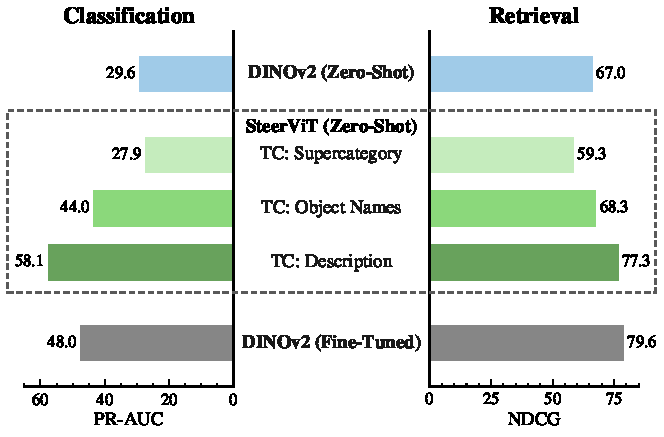
\includegraphics[width=\textwidth]{figures/personalized_representations_back_to_back.pdf}
    % \caption{XXXX}
\end{subfigure}
\begin{subfigure}[b]{0.50\textwidth}
    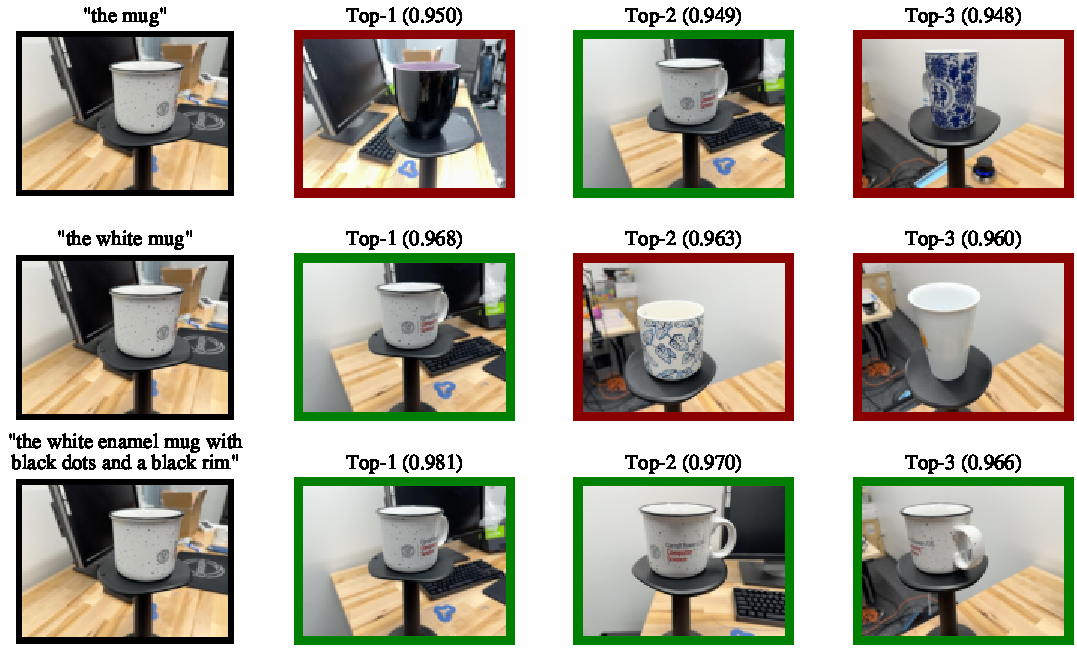
\includegraphics[width=\textwidth]{figures/personalized_representations_retrieval_comparison.pdf}
    % \caption{XXXX}
\end{subfigure}
\caption{\textbf{Text specificity controls feature granularity.} \textbf{Left:} \JR{TODO: make lines and text bigger on left plot}
The quality of personalized representations produced by \model{} improves drastically with more detailed prompts, even surpassing a supervisedly fine-tuned DINOv2.
\textbf{Right:} Qualitative example showing better retrievals when providing \model{} with more detailed descriptions.
\MT{need to add query in col 1 and may be draw separator lines to indicate how to read this. also, can reduce gaps between figures or make them bigger I guess; hard to see the design on the mug at 100\% right now}
}
\label{fig:pods}
\end{figure}

\cref{subsec:cond_ret_exp} showed that the conditioning text has a profound impact on the resulting features; conditioning on a random object class halved retrieval performance.
Here, we systematically explore the role of text in forming high-fidelity visual representations.
% In this section, we systematically explore how text steers our visual representation.

We do this using the Personal Object Discrimination Suite (PODS)~\cite{sundaram2024personalized_pods}, a benchmark evaluating the formation of instance-aware feature spaces via the ability of models to recognizing specific instances of objects (e.g., ``your'' mug vs. all other mugs).
Given a small set of reference images, PODS computes cosine similarities on frozen global features and performs:
(i)~one-vs-all instance classification as well as
(ii)~similarity-based retrieval over a set of test images.
% under distribution shifts.
Following~\cite{sundaram2024personalized_pods}, we report PR-AUC and NDCG scores for classification and retrieval respectively. 


\subsubsection{From coarse to fine-grained steering.}

We vary the amount of detail provided to \model{} via the text prompt from
coarse supercategories (e.g., ``mug'', ``shoe''), 
object names (e.g., ``white ECCV mug''),
to comprehensive descriptions of each instance's visual appearance. 
\MT{are these descriptions manual / MLLM?}
As shown in \cref{fig:pods}, the semantics of the steered representations are highly sensitive to the prompt specificity.
Coarse conditioning ignores specific lower-level cues relevant for discriminating instances within an object type, resulting in worse performance than vanilla DINOv2.
Increasing the prompt detail drastically improves performance, allowing \model{} to outperform custom DINOv2 variants fine-tuned on (synthetic) instance data in the classification setting.
\MT{might be good to add some numbers like in sec 4.2}

These results demonstrate that the model does not simply \textit{add} information to the underlying visual encoder but instead precisely steers the feature space to match the prompt-provided level of detail.
\JR{Not sure if to include the following:} This aligns with Figure~\ref{fig:ref4_token_len} (Appendix), where referential segmentation accuracy increases monotonically with caption length, confirming that denser text yields more precise steering.
\MT{yeah, ok to skip} \MG{can also say (also illustrated in Supplementary)}

% This demonstrates that natural language can steer features effectively in out-of-distribution domains where labeled data for fine-tuning is scarce. \MG{can drive a strong point in conjuction with anomaly detection results}


\subsection{Visualizing and Analyzing Steered Embedding Space}
\label{sec:tsne_viz}

The results on PODS (\cref{subsec:text_density_exp}) indicate that query specificity dictates the level of semantic abstraction.
Next, we visualize how text conditioning shapes the embedding space topology of \model{} using two complementary modes: steering along the \textit{semantic hierarchy} and steering by \textit{compositional attributes}.

For this, we select XXX\JR{fill once final} images containing exactly one out of XXX\JR{fill once final} curated classes from PASCAL-VOC~\cite{pascal_voc}. The encoded global image features are then reduced to 2D using UMAP~\cite{}\JR{citation}. 


% We test whether text can steer clustering at different levels of the semantic hierarchy, from object class (``bird'') to generic superclass (``animal'').

\subsubsection{Steering Along the Semantic Hierarchy.}
% While DINOv2 imposes a fixed topology dictated by the semantic relatedness of salient objects, \model{} dynamically reorganizes it according to the text query.
As shown in Figure~\ref{fig:tsne_semantic} (panel~1), DINOv2 embeddings cluster rigidly by object class.
Conditioned on \texttt{``animal''} (panel~2), two macro-clusters emerge for \model{}, containing all animal and non-animal classes, respectively. Crucially, fine-grained structure is preserved (e.g., dogs and cats remain closer than birds), confirming that text controls clustering granularity without destroying object-level semantics.
Drilling down further, conditioning on \texttt{``bird''} (panel~3) increases separability between bird and non-bird images while preserving the higher-level animal versus non-animal macro-separation.
This confirms that text can steer clustering at multiple levels of the semantic hierarchy. \YA{maybe say this is emergent, as we only trained with random data we f0ound}

% --- Old text (commented out) ---
% \subsubsection{Steering Feature along the Semantic Hierarchy}
% This experiment tests whether text can steer clustering using different levels of semantic details, ranging from low level fine-grained object description (as seen in ~\cref{subsec:text_density_exp}) to higher level semantics i.e object class (``bird'') and generic semantic superclass (``animal'').
% \paragraph{Setup.} We select images containing $N$ distinct object classes divided into $k$ object classes.
% \paragraph{Analysis.} 
% As shown in Figure~\ref{fig:tsne_semantic}, the baseline DINOv2 embeddings (left) form six distinct clusters, rigidly adhering to object class and treating ``dog'' and ``horse'' as separate concepts.
% Conditioning our model on \texttt{``Animal''} (right) transforms the embedding space: all animal classes (dog, cat, horse, bird, sheep) collapse into a single macro-cluster, while non-animal classes are pushed away.
% Crucially, object-level semantics are preserved within the animal cluster: dogs and cats remain closer neighbors than birds (Figure~\ref{fig:tsne_semantic}), confirming that text controls the granularity of clustering without destroying fine-grained structure.


\begin{figure}[t]
\centering
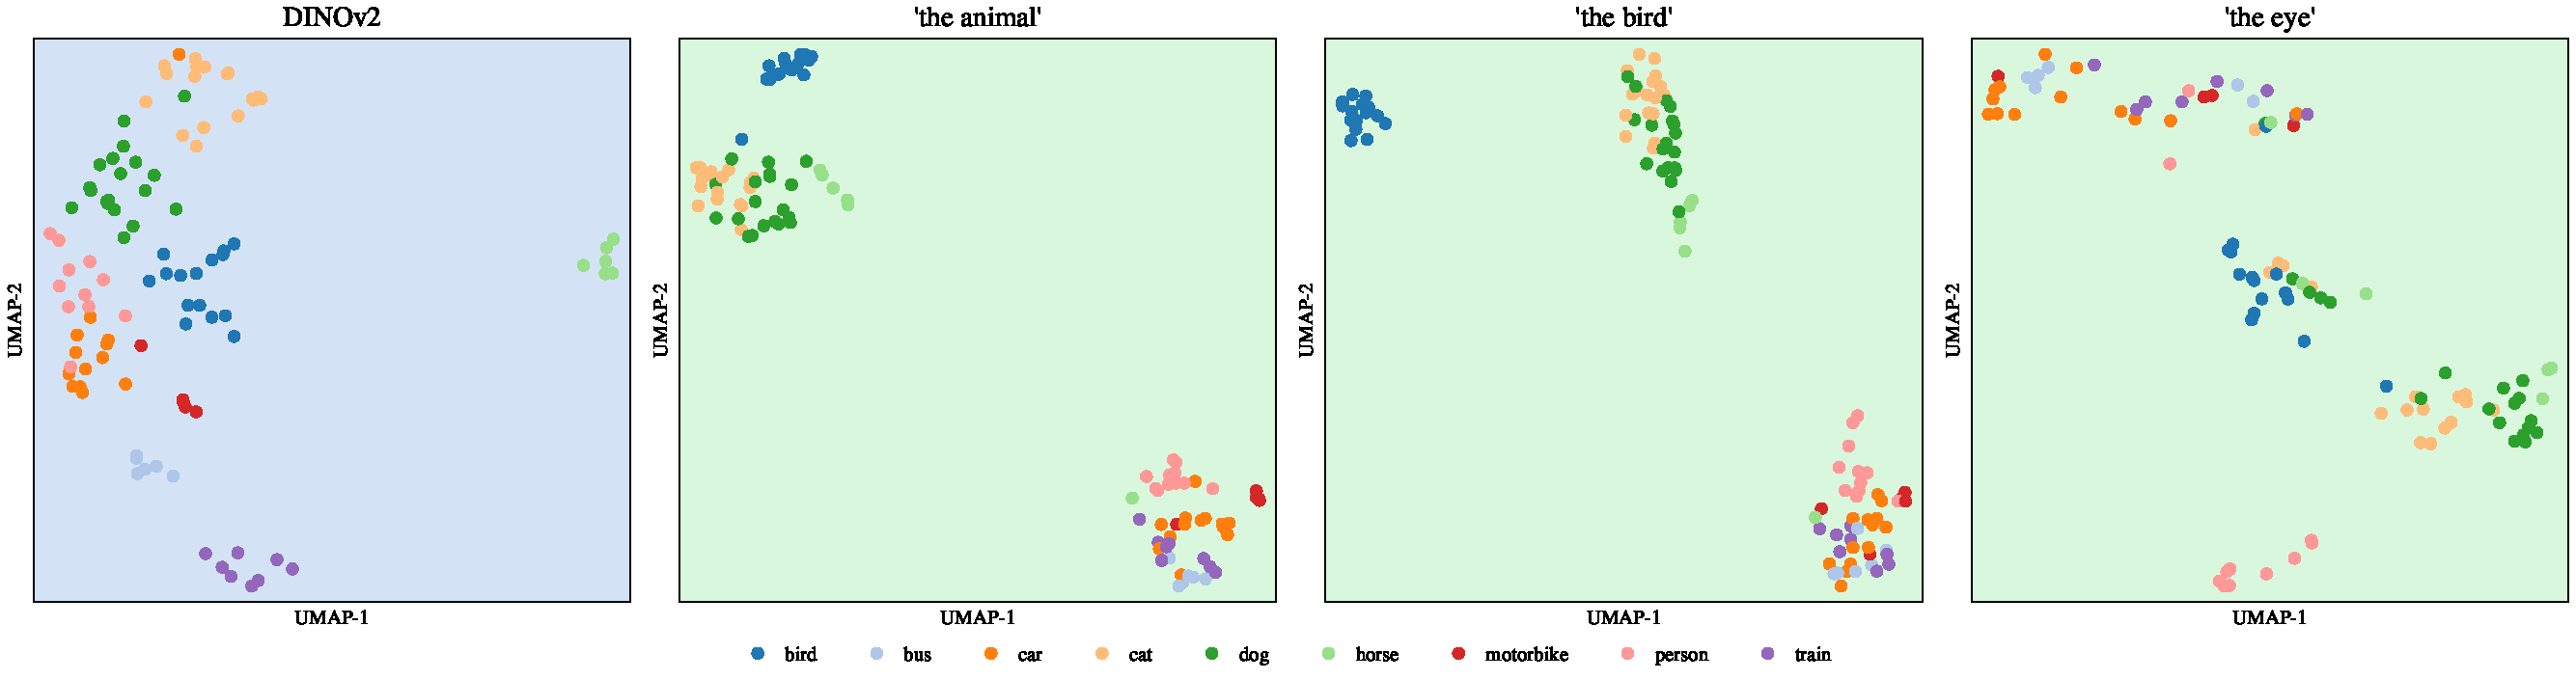
\includegraphics[width=\linewidth]{figures/tsne_animal.pdf}
\caption{\textbf{\model{} steers embedding topology via text.}
\textbf{(1)} DINOv2 clusters by object class.
\textbf{(2)} Conditioning on \texttt{``animal''} merges animal classes into one cluster while separating non-animals.
\textbf{(3)} Conditioning on \texttt{``bird''} increases bird vs.\ non-bird separability while preserving the animal/non-animal macro-structure.
\textbf{(4)} Conditioning on \texttt{``eye''} groups all animate classes (including person) together, demonstrating compositional attribute steering.
\JR{plot is not final; caption needs adaptation}
\YA{again make some circles around area that reader should look at. }}
% --- Old caption (commented out) ---
% \caption{\textbf{\model{} enables hierarchical semantic steering.} \textbf{(1)} DINOv2 clusters images by object class. \textbf{(2)} Conditioning \model{} on \texttt{``animal''} separates images into animal and non-animal clusters. \textbf{(3)} \JR{potentially remove this hierarchy level} \textbf{(4)} With \texttt{``eye''}-conditioning, two primary clusters containing animate and inanimate classes emerge. \JR{plot is not final; caption needs adaptation}}
\label{fig:tsne_semantic}
\end{figure}

\subsubsection{Steering by Compositional Attributes.}
Besides semantic categories, it is also possible to steer by compositional attributes, i.e., shared sub-object properties. This defines an grouping principle orthogonal to semantic categories.
Conditioning on \texttt{``eye''} (Figure~\ref{fig:tsne_semantic}, panel~4) produces two macro clusters: animate classes that possess eyes versus inanimate objects that do not.
Notably, \textit{person} images, which were distant from animals under both \texttt{``animal''} and \texttt{``bird''} conditioning, now join the animate cluster since the shared attribute ``has eyes'' overrides the semantic category boundary.
This demonstrates that \model{} can steer representations by compositional properties, not just taxonomic ones.

\MT{will take a pass again after finalizing results}

% --- Old "wheel" experiment (commented out) ---
% \subsubsection{Steering Feature along the Object Composition Hierarchy}
%
% This experiment tests a more challenging scenario: clustering visually dissimilar objects (e.g., office chair and bike) based on a shared sub-object attribute (wheel), ignoring their primary semantic category.
%
% \paragraph{Setup.} We curate a heterogeneous dataset split into two compositional groups:
% \begin{itemize}
% \item \textbf{Has-Part ``Wheel'':} Cart, wheelchair, bike, car, airplane.
% \item \textbf{No-Part ``Wheel'':} Apple, house, person.
% \end{itemize}
%
% \paragraph{Analysis.} 
% DINOv2 fails to capture this shared attribute: the t-SNE visualization (Figure~\ref{fig:tsne_compositional}, left) shows clusters organized by object identity, with a wheelchair clustered closer to a person (contextual bias) than to a cart.
%
% Conditioning on \texttt{``Wheel''} produces a binary separation of the embedding space (Figure~\ref{fig:tsne_compositional}, right): one cluster containing all objects with wheels, regardless of whether they are vehicles or medical equipment, and another containing objects without wheels.
% This confirms that text conditioning can route attention to specific compositional attributes rather than the global object concept.
% \begin{figure}[t]
% \centering
% % \includegraphics[width=\linewidth]{old_figures/tsne_compositional_steering.png}
% \caption{\textbf{Compositional attribute steering.} \textbf{Left:} DINOv2 separates objects by class (wheelchair far from car). \textbf{Right:} Conditioned on \texttt{``Wheel''}, our method clusters diverse wheeled objects together (cart, wheelchair, car), distinct from objects without wheels (apple, house).}
% \label{fig:tsne_compositional}
% \end{figure}

% TODO: Impact of varying text density
% TODO: Impact of turning down the Cross Attention knob


% ------------------------------------------------------------

\subsection{Text Facilitates Zero-Shot Domain Transfer}



The previous sections established that \model{} steers global features with text, routes attention to queried concepts, and preserves representation quality of the underlying ViT.
We now ask: \textit{Does this combination enable generalization to domains unseen during training?} \JR{Feel like this is not motivated well enough yet. Doesn't feel like the most natural question to ask next. Maybe we can refer to literature saying language helps robustness in CLIP-like models?! (Although quite contested and confounded by data)}
We evaluate this aspect in two progressively harder out-of-distribution settings: personalized instance recognition via PODS (natural images of novel object instances with camera distribution shifts) and industrial anomaly segmentation.

\subsubsection{Personalized Object Discrimination: OOD Task Transfer.}
% The results on PODS in Section~\ref{subsec:text_density_exp} show that text specificity controls feature granularity on the PODS benchmark.
A surprising result emerging from the analysis of PODS performance in Section~\ref{subsec:text_density_exp} is that, when utilizing descriptive text prompts, \model{} not only adapts to this novel task setup zero-shot but outperforms the specialized DINOv2 variants fine-tuned on instance-specific data (58.3\% vs. 48.0\% PR-AUC).
\MT{not so on retrieval though .. someone may point out; can we pre-empt this?}
% Frozen DINOv2 scores 29.6\% AUPRC on PODS; supervised fine-tuning on synthetic instance  more than doubles this to 48.0\%; yet our method reaches 58.3\% without seeing a single labeled example from the target domain (Figure~\ref{fig:pods}).
In comparison, CLIP and SigLIP with late text fusion only achieve 26.7\% and 16.4\%, respectively. 
This illustrates that generalization to this task requires both a rich frozen vision encoder and early text conditioning while preventing overwriting of general-purpose features as might occur during fine-tuning. 

% also fail on this task, confirming that OOD generalization requires both a rich frozen vision encoder and early text conditioning. \MG{poor writing}
% Text conditioning in our method succeeds here because it steers the frozen encoder's rich representations without catastrophic forgetting; fine-tuning, by contrast, overwrites general features with task-specific ones.
% Just as in-context learning adapts language models to novel tasks at inference time, text prompts adapt visual representations to novel domains without retraining. 


\subsubsection{Anomaly Segmentation: Extreme OOD Domain Transfer.}
In addition to generalizing to novel tasks like PODS, we showcase \model{}'s adaptability by performing anomaly segmentation (AS) on the MVTec~AD~\cite{bergmann_mvtech} dataset containing industrial images never seen during training with the goal of identifying subtle manufacturing defects or irregularities.
\MT{we should briefly describe what text prompt is used}
We derive anomaly maps by upsampling the heatmap produced by the learned linear segmentation head and compare to other segmentation models as well as other dedicated AS methods using \textit{Per-Region-Overlap} (PRO). 
As shown in Figure~\ref{} (Right)\JR{TODO}, \model{} again matches dedicated zero-shot methods on this extreme OOD setting.
These results further reinforce the pattern of text-driven steering unlocking capabilities already present in the frozen ViT and transferring them to domains beyond the training distribution.


\JR{Will add a qualitative Figure showing examples of anomaly heatmaps and might change table to Figure (or at least only consider MVTech)}
\JR{Will probably add a qualitative Figure showing examples of anomaly heatmaps}


% Having established OOD generalization on natural images, we escalate the domain gap to industrial anomaly detection. It requires localizing subtle manufacturing defects in factory inspection imagery.
% , a domain entirely absent from our training data.


% \iffindingbox
% \begin{tcolorbox}[colback=lightyellow,
% colframe=black, arc=4pt, boxsep=1pt]
% \paragraph{\textbf{\textit{Finding} 4.}}
% Natural language serves as a data-efficient generalization mechanism
% % : descriptive text prompts 
% adapting 
% % frozen visual representations 
% the visual encoder
% to out-of-distribution domains without task-specific training \JR{would remove the following since AS is zero-shot and it's a pretty strong claim in general}, outperforming supervised fine-tuning.
% % on personalized object discrimination and matching dedicated methods on industrial anomaly detection.\
% \YA{finding sounds a bit overblown: the finding is just that text even allows extreme OOD transfer. I don't see any evidence for "data-efficiency" and "adapting the visual encoder to out-of-distribution domains without .. training" sounds odd. }
% \end{tcolorbox}
% \fi

% \begin{table*}[t]
\centering
\footnotesize
\setlength{\tabcolsep}{4pt}
% \renewcommand{\arraystretch}{1.15}
\begin{threeparttable}
\caption{Zero-shot segmentation performance on industrial AD data.}
\label{tab:mvtec_visa}
\begin{tabular}{l l c
                S[table-format=2.1] S[table-format=2.1] S[table-format=2.1]
                S[table-format=2.1] S[table-format=2.1] S[table-format=2.1]}
\toprule
\multicolumn{3}{c}{\textbf{Method}} &
\multicolumn{3}{c}{\textbf{MVTec AD}} &
\multicolumn{3}{c}{\textbf{VisA}} \\
\cmidrule(lr){1-3}\cmidrule(lr){4-6}\cmidrule(lr){7-9}
Name & Ref. & AD &
{$\text{ROC}_P$} & {PRO} & {$F_1^{\max}$} &
{$\text{ROC}_P$} & {PRO} & {$F_1^{\max}$} \\
\midrule
% TransMM  & \cite{Chefer_2021_transmm} & \xmark & 57.5    & 21.9    & 12.1   & 49.4   & 10.2   & 3.1    \\
MaskCLIP & \cite{zhou2022_maskclip} & \xmark & 63.7    & 40.5    & 18.5   & 60.9   & 27.3   & 7.3    \\
CLIPseg  & \cite{lueddecke22_clipseg} & \xmark & 69.0    & 34.6    & 12.5   & 89.5   & 62.4   & 13.9   \\
SAM3     & \cite{carion2025_sam3} & \xmark & 79.9    & 54.5    & 24.1   & 89.8   & 65.9   & 15.5   \\
\addlinespace
\color{gray}WinCLIP  & \color{gray}\cite{WinCLIP_Jeong23CVPR} & \color{gray}\cmark & \color{gray}85.1    & \color{gray}64.6    & \color{gray}31.7   & \color{gray}79.6   & \color{gray}59.8   & \color{gray}14.8   \\
% AnoCLIP  & \cite{deng2024_anoclip} & \cmark & 86.6    & 70.4    & 30.1   & 85.9   & 65.1   & 14.7   \\
% SDP      & \cite{chen2023_clipad} & \cmark & 87.5    & 75.3    & 35.9   & 88.1   & 68.5   & 17.0   \\
% SAA+     & \cite{cao_2023_saa} & \cmark & 73.2    & 42.8    & \underline{37.8}   & 74.0   & 36.8   & \textbf{27.1}   \\
\color{gray} DIVAD    & \color{gray}\cite{hicsonmez2026training}& \color{gray} \cmark & \color{gray}88.0    & \color{gray}72.5    & \color{gray}\underline{35.5}   & \color{gray}\textbf{93.4}   & \color{gray}\underline{78.2}   & \color{gray}\textbf{24.0}   \\
\color{gray}FADE     & \color{gray}\cite{li2024_fade} & \color{gray}\cmark & \color{gray}\textbf{89.6}    & \color{gray}\textbf{84.5}    & \color{gray}\textbf{39.8}   & \color{gray}\underline{91.5}   & \color{gray}\textbf{79.3}   & \color{gray}16.7   \\
\addlinespace
\rowcolor{\methodcolor}\textbf{SHIFT} & \textbf{Ours} & \xmark & \underline{88.1} & \underline{79.4} & 32.6 & \underline{91.5} & 77.5 & \underline{16.9} \\
\bottomrule
\end{tabular}

\begin{tablenotes}[flushleft]\footnotesize
\item AD indicates dedicated anomaly detection methods.
% \item \textdagger{} indicates results reported in one of \cite{WinCLIP_Jeong23CVPR, hicsonmez2026training,chen2023_clipad, deng2024_anoclip}. %mark with \textsuperscript{\textdagger}
\end{tablenotes}
\end{threeparttable}
\end{table*}


% \section{Applications}
% \subsection{Anomaly Detection}

% We further evaluate SHIFT's robustness and dense localization capabilities by performing zero-shot anomaly segmentation (AS) on the MVTech AD \cite{bergmann_mvtech} and VisA \cite{zou2022_visa_dataset} datasets for industrial anomaly detection (AD).

% For SHIFT, we derive the anomaly map by upsampling the continuous heatmap produced by the learned linear segmentation head. As for all text-steerable methods, we use an ensemble of ten anomaly prompts (e.g., \texttt{``the anomaly in the <object>.''}) and average the resulting heatmaps across prompts.
% % For text-steerable segmentation method such as SHIFT, we apply an ensemble of ten anomaly-related prompts (e.g., \texttt{``the anomaly in the <object>.''}) and average the resulting continuous heatmaps across prompts. 
% Following standard practice in the AD literature \cite{WinCLIP_Jeong23CVPR}, we measure the pixel-wise \textit{Area under the Receiver Operating Characteristics} ($\text{ROC}_P$), the \textit{Per-Region-Overlap} (PRO), and threshold-optimal $F_1$ score ($F_1^{\max}$). Performance of existing training- and adaptation-free AS baselines is stated as reported in the original publication. 

% Despite its general-purpose nature, \model{} is competitive with dedicated AS approaches. As shown in Table~\ref{tab:mvtec_visa}, it reaches 79.4 PRO on MVTech AD, substantially improving over prompt-based non-AD baselines (e.g., SAM3 at 54.5) and closing much of the gap to specialist methods (e.g., FADE at 84.5). Similar trends appear on VisA, indicating robust transfer to a harder, more diverse inspection setting. Overall, these results suggest that SHIFT’s text-driven post-training unlocks dense visual capabilities already present in the frozen ViT, yields strong out-of-domain generalization to industrial AD tasks without any task-specific training.\todo{use final numbers}

% \begin{table*}[t]
\centering
\footnotesize
\setlength{\tabcolsep}{4pt}
% \renewcommand{\arraystretch}{1.15}
\begin{threeparttable}
\caption{Zero-shot segmentation performance on industrial AD data.}
\label{tab:mvtec_visa}
\begin{tabular}{l l c
                S[table-format=2.1] S[table-format=2.1] S[table-format=2.1]
                S[table-format=2.1] S[table-format=2.1] S[table-format=2.1]}
\toprule
\multicolumn{3}{c}{\textbf{Method}} &
\multicolumn{3}{c}{\textbf{MVTec AD}} &
\multicolumn{3}{c}{\textbf{VisA}} \\
\cmidrule(lr){1-3}\cmidrule(lr){4-6}\cmidrule(lr){7-9}
Name & Ref. & AD &
{$\text{ROC}_P$} & {PRO} & {$F_1^{\max}$} &
{$\text{ROC}_P$} & {PRO} & {$F_1^{\max}$} \\
\midrule
% TransMM  & \cite{Chefer_2021_transmm} & \xmark & 57.5    & 21.9    & 12.1   & 49.4   & 10.2   & 3.1    \\
MaskCLIP & \cite{zhou2022_maskclip} & \xmark & 63.7    & 40.5    & 18.5   & 60.9   & 27.3   & 7.3    \\
CLIPseg  & \cite{lueddecke22_clipseg} & \xmark & 69.0    & 34.6    & 12.5   & 89.5   & 62.4   & 13.9   \\
SAM3     & \cite{carion2025_sam3} & \xmark & 79.9    & 54.5    & 24.1   & 89.8   & 65.9   & 15.5   \\
\addlinespace
\color{gray}WinCLIP  & \color{gray}\cite{WinCLIP_Jeong23CVPR} & \color{gray}\cmark & \color{gray}85.1    & \color{gray}64.6    & \color{gray}31.7   & \color{gray}79.6   & \color{gray}59.8   & \color{gray}14.8   \\
% AnoCLIP  & \cite{deng2024_anoclip} & \cmark & 86.6    & 70.4    & 30.1   & 85.9   & 65.1   & 14.7   \\
% SDP      & \cite{chen2023_clipad} & \cmark & 87.5    & 75.3    & 35.9   & 88.1   & 68.5   & 17.0   \\
% SAA+     & \cite{cao_2023_saa} & \cmark & 73.2    & 42.8    & \underline{37.8}   & 74.0   & 36.8   & \textbf{27.1}   \\
\color{gray} DIVAD    & \color{gray}\cite{hicsonmez2026training}& \color{gray} \cmark & \color{gray}88.0    & \color{gray}72.5    & \color{gray}\underline{35.5}   & \color{gray}\textbf{93.4}   & \color{gray}\underline{78.2}   & \color{gray}\textbf{24.0}   \\
\color{gray}FADE     & \color{gray}\cite{li2024_fade} & \color{gray}\cmark & \color{gray}\textbf{89.6}    & \color{gray}\textbf{84.5}    & \color{gray}\textbf{39.8}   & \color{gray}\underline{91.5}   & \color{gray}\textbf{79.3}   & \color{gray}16.7   \\
\addlinespace
\rowcolor{\methodcolor}\textbf{SHIFT} & \textbf{Ours} & \xmark & \underline{88.1} & \underline{79.4} & 32.6 & \underline{91.5} & 77.5 & \underline{16.9} \\
\bottomrule
\end{tabular}

\begin{tablenotes}[flushleft]\footnotesize
\item AD indicates dedicated anomaly detection methods.
% \item \textdagger{} indicates results reported in one of \cite{WinCLIP_Jeong23CVPR, hicsonmez2026training,chen2023_clipad, deng2024_anoclip}. %mark with \textsuperscript{\textdagger}
\end{tablenotes}
\end{threeparttable}
\end{table*}


\input{sections/5_ablation}
\input{sections/6_conclusion}


% \bibliography{bib/longstrings,bib/refs}
% \bibliographystyle{tmlr}

% \appendix
% % \input{sections/X_appendix}








% ---- Bibliography ----
%
% BibTeX users should specify bibliography style 'splncs04'.
% References will then be sorted and formatted in the correct style.
%
\bibliographystyle{splncs04}
\bibliography{main}
\end{document}
